
\documentclass[11pt,twoside,a4paper]{book}

\newcommand{\sphere}{\mathds{S}^{d-1}}
\newcommand{\esfera}{\mathds{S}^{2}}
\newcommand{\orto}{\mathds{O}^d}
\newcommand{\R}{\mathds{R}^d}
\newcommand{\spharm}{\mathds{Y}^d_n}
\newcommand{\sphint}{\int_{\sphere}}
\usepackage[spanish,activeacute]{babel} % Para poner acentos y ñ en español
\usepackage[T1]{fontenc}
\usepackage[utf8]{inputenc}
\usepackage{lmodern}
\usepackage{amsmath}
\usepackage{amsthm}
\usepackage{amssymb}
\usepackage{latexsym}
\usepackage{graphicx}
\usepackage{enumerate}   
\usepackage[hidelinks=true]{hyperref}
\usepackage{dsfont}
\usepackage{appendix}
\usepackage{graphicx}
\usepackage{float}
\usepackage{algorithm}
\usepackage{algorithmic}
%Numeracion de teoremas, proposiciones, etc.
\numberwithin{equation}{section}
\numberwithin{figure}{section}
\theoremstyle{plain}
\newtheorem{thm}{Teorema}[chapter]
  \theoremstyle{definition}
        \newtheorem{defn}[thm]{Definici\'{o}n}
        \theoremstyle{plain}
  \newtheorem{prop}[thm]{Proposici\'{o}n}
        \theoremstyle{definition}
        \newtheorem{example}[thm]{Ejemplo}
  \theoremstyle{remark}
        \newtheorem{rem}[thm]{Nota}
  \theoremstyle{definition}
        \newtheorem{problem}[thm]{Problema}
  \theoremstyle{lem}
	  \newtheorem{lem}[thm]{Lema}
  \theoremstyle{cor}
  \newtheorem{cor}[thm]{Corolario}

\setlength{\oddsidemargin}{2cm}
\setlength{\evensidemargin}{1cm}

\DeclareGraphicsExtensions{.jpg,.pdf,.mps,.png}

\pagestyle{empty}

\begin{document}


\thispagestyle{empty}

%Portada

\begin{center}

%{\Large UNIVERSIDAD DE GRANADA}\\[8mm]
%{\Large Facultad de Ciencias}\\[8mm]

\includegraphics[width=9cm]{simbolo_color.png}\\[2cm]
{\Large\sffamily M\'aster Universitario en F\'isica y Matem\'aticas}\\[3mm]


\vspace{2cm}


\begin{Large}
{\slshape\bfseries  EL T\'ITULO DEL TRABAJO\\[6mm]
FIN DE M\'ASTER}
\end{Large}

\vspace{2cm}

\vfill

\begin{large}
{\bf Trabajo Fin de M\'aster presentado por \\[3mm]
Nombre Apellido1 Apellido2}
\end{large}


\vspace{1.5cm}

\begin{Large}
Curso 2016/17
\end{Large}
\end{center}




%%%%%%%%%%%%%%%%%%%%%%%%% Página en blanco, revés de la primera página

\quad

\thispagestyle{empty}


\newpage 

%%%%%%%%%%%%%%% Página de portada


\thispagestyle{empty}


\begin{center}

{\Large UNIVERSIDAD DE GRANADA}\\[10mm]
%{\Large Facultad de Ciencias}\\[4mm]
%\includegraphics[width=4cm]{escudo_ugr}\\[4mm]
{\Large\sffamily M\'aster Universitario en F\'isica y Matem\'aticas}\\[3mm]


\vspace{3cm}


\begin{Large}
{\slshape\bfseries  EL T\'ITULO DEL TRABAJO\\[6mm]
FIN DE M\'ASTER}
\end{Large}

\vspace{3cm}

\vfill

\begin{large}
{\bf Trabajo Fin de M\'aster presentado por \\[3mm]
Nombre Apellido1 Apellido2}
\end{large}


\vspace{2cm}

\begin{Large}
Curso 2016/17
\end{Large}
\end{center}

\vfill

\noindent
Tutor: Nombre Apellido1 Apellido2

\noindent
Departamento: Matem\'atica Aplicada

\noindent
\'Area de Conocimiento: Matem\'atica Aplicada

\newpage

%%%%%%%%%%%% Página en blanco, revés

\thispagestyle{empty}

\quad

\newpage

\thispagestyle{empty}

\vspace*{2cm}

\begin{flushright}
\parbox{3.5in}
{\small
(P\'agina de agradecimientos si los hay)


Thank you.}

\end{flushright}

\newpage




\newpage
\phantom{o}
\newpage

\pagenumbering{roman}
\setcounter{page}{3}

\renewcommand{\contentsname}{Índice}
\tableofcontents

\newpage
\phantom{o}
\newpage

\pagestyle{headings}

\setcounter{page}{1}
\pagenumbering{arabic}

%Si quieres poner tus propias marcas en el borde superior de las páginas
%\pagestyle{myheadings}
%\def\leftmark{\textsc{Nombre del autor}}
%\def\rightmark{\textsc{Trabajo Fin de Grado}}

\renewcommand{\appendixname}{Apéndices}
\renewcommand{\appendixtocname}{Apéndices}
\renewcommand{\appendixpagename}{Apéndices}

%Cuerpo del trabajo, se incluye por cap´itulos

%\chapter*{Introducción}
\subsection*{Summary}

In this work, we consider systems of points on the unit sphere related to problems of approximation and numerical integration. This sistems are useful in various fields ranging from global climate models for the Earth, mapping of the stationary and magnetic fields of the Earth, crystallography, geodesic domes, virus modeling, computational geometry, etc.
\medskip

Starting with the construction of the spherical armonic space. Next, we study the Addition Theorem and its consequences. This result will allow us to generate an	 orthonormal basis of the space of spherical harmonics. 
Later, we get an expression for critical points of the gradient of a sherical armonic. In particular, we get critical points of the 3-dimensional sphere. 

Finally, we get some results about numeric quadrature.

\medskip
In the second part of the work, we explain the process followed for participation in a data mining competition. This process consists of the parts related to the understanding of the problem, the visualization of the data with which we will work, the application of preprocessing techniques to improve the data set and the choice of the algorithm to use to build a data model . Finally, we discuss the results obtained.

\bigskip
\emph{keywords:} sphere, spherical armonic, gradient, preprocessing, machine learning.
\newpage
\subsection*{Resumen}
Uno de los propósitos de este trabajo es determinar conjuntos de puntos para aproximación, interpolación e integración sobre la esfera y sus propiedades geométricas. Las distribuciones de puntos en la esfera unidad tienen aplicaciones que van desde modelos climáticos globales para la  Tierra, mapeado de los campos estacionales y magnéticos de la Tierra, cristalografía, cúpulas geodésicas, modelado de virus, geometría computacional, etc.

\medskip
Para ello, en primer lugar, introduciremos de forma constructiva el espacio de los armónicos esféricos sobre el que trabajaremos. Una vez construido dicho espacio, trataremos el Teorema de adición y sus consecuencias. Estos ingredientes nos permitirán generar una base ortonormal del espacio de esféricos armónicos.

Una vez asentadas las bases, estudiaremos el gradiente de dichos polinomios y calcularemos sus puntos críticos. Como caso particular, estudiaremos los puntos críticos de dichos polinomios sobre la esfera de dimensión tres y obtendremos una visualización de los resultados obtenidos.

Finalmente, trataremos varios resultados sobre integración numérica.
\bigskip

En la segunda parte del trabajo, explicaremos el proceso seguido durante la participación en una competición de data mining. Dicho proceso consta de las partes relativas a la comprensión del problema, la visualización de los datos con los que vamos a trabajar, la aplicación de técnicas de preprocesamiento para mejorar el conjunto de datos y la elección del algoritmo a usar para construir un modelo de datos. Finalmente, estudiaremos los resultados obtenidos y realizaremos un análisis sobre los mismos. 
	
\bigskip
\emph{Palabras clave:} esfera, armónicos, gradiente, preprocesamiento, clasificación.
\newpage


\subsection*{Objetivos.}
Los objetivos propuestos al inicio del trabajo fueron los siguientes:
\begin{itemize}
	\item Simulación y visualización de distribuciones de puntos sobre la esfera
	\item Estimación numérica de la calidad de las aproximaciones obtenidas mediante estas distribuciones de puntos. 
	\item Enfrentarse a un problema real de machine learning, estudiando las posibles soluciones y los resultados obtenidos.
\end{itemize}

El primer objetivo se ha logrado satisfactoriamente, siendo desarrollado en el Capítulo 2. El segundo objetivo se ha alcanzado durante el desarollo del Capítulo 3. Finalmente, el tercer objetivo se ha cumplido, siendo desarrollado en la segunda parte del trabajo.

\subsection*{Organización de la memoria.}
\medskip

El Capítulo 1 contiene todo lo referente a la definición y construcción del espacio de polinomios armónicos esféricos.
En el Capítulo 2 se calculará el gradiente de dichos polinomios y se estudiarán sus puntos críticos. Se estudiará el caso particular de dimensión 3, obteniendo una visualización de los puntos obtenidos sobre la esfera.
Finalmente, en el capítulo 3 se estudiaran diferentes resultados de integración numérica.
\medskip

En cuanto a la segunda parte del trabajo, en el Capítulo 4 se realiza una introducción al problema a tratar. 
En los Capítulos 5 y 6 se describe el proceso de visualización y posterior preprocesamiento del conjunto de datos.
En el Capítulo 7 se describen los algoritmos usados para resolver el problema.
Finalmente, en el Capítulo 8 se resumen los resultados obtenidos y se describen las conclusiones obtenidas.

\medskip 

Para la redacción de los Capítulos 1 y 3 se ha tomado como referencia \cite{libro_esfarm}, mientras que en el Capítulo 2 se ha tomado como referencia \cite{art_grad}. Para la segunda parte del trabajo se han tomado como referencia los libros \cite{data_mining} y \cite{clasification}. Además, para desarrollar el Capítulo 7 se ha tomado como referencia \cite{boosting}, \cite{rusboost} y \cite{cusboost}. 
\chapter[Esféricos Armónicos]
        {Esféricos Armónicos}
\section{Preliminares}
\subsection{Notación}
Para empezar fijaremos la notación que seguiremos durante el capítulo. Usaremos $d\in\mathds{N}$ para representar la dimensión de un conjunto; en particular, el conjunto $\mathds{R}^d = \{x=(x_1,...,x_d)^T : x_j\in\mathds{R},1 \le j \le d\}$ es el espacio euclídeo de dimensión d con el producto escalar y la norma definidos por
$$
(x,y) = \sum_{j=1}^{d} x_jy_j  \qquad |x|=(x,x)^{1/2}  \qquad x,y\in\mathds{R}^d
$$
En $\mathds{R}^d$ usaremos la base canónica
$$
e_1=(1,0,...,0)^T, ..., e_d=(0,0,...,1)^T
$$
y escribiremos $x = \sum_{j=1}^{d} x_je_j, x\in\mathds{R}^d$.
\medskip

Para indicar la dimensión explícitamente usaremos $x_{(d)}$ en lugar de $x$. En tal caso, $x_{(d)} = x_{(d-1)}+x_de_d$ siendo $x_{(d-1)}=(x_1,...,x_{d-1},0)^T$. También usaremos $x_{(d-1)}$ para referirnos al vector (d-1)-dimensional $(x_1,...,x_{d-1})^T$.
\medskip

Trabajaremos sobre la esfera unidad $\sphere = \{\xi\in\R : |\xi| = 1\}$. Por simplicidad, llamaremos esfera a $\sphere$.
\begin{defn} Sean $\xi,\eta\in\mathds{S}^{d-1}$, definimos las siguientes distancias:
	\begin{itemize}
		\item La distancia euclídea $|\xi-\eta| = \sqrt{2(1-\xi\cdot\eta)}$
		\item La distancia geodésica $\theta(\xi,\eta)=\arccos(\xi.\eta)$
	\end{itemize}	
\end{defn}

\begin{rem}Usando que $\frac{2}{\pi} \le \sen t \le t,t\in[0,\pi/2]$ se deduce la siguiente relación entre ambas distancias:
	$$
	\frac{2}{\pi}\theta(\xi,\theta) \le |\xi - \eta| \le \theta(\xi,\eta)
	$$ 
esto es, ambas distancias son equivalentes.
\end{rem}

Para $x =(x_1,...,x_d)$ definimos $x^\alpha = x_1^{\alpha_1}...x_d^{\alpha_d}$. Análogamente,
para el operador gradiente $\triangledown = (\partial_{x_1},...,\partial_{x_d})^T$ definimos
$$
	\nabla^\alpha = \frac{\partial^{|\alpha|}}{\partial x_1^{\alpha_1}...\partial x_d^{\alpha_d}}
$$
Y finalmente definimos el operador laplaciano como
$$ 
	\triangle = \nabla.\nabla = \sum_{j=1}^{d}(\frac{\partial}{\partial x_j})^2
$$


%\begin{defn} Dado $x\in\mathds{(R)^+}$ definimos la función gamma como
%	$$
%	\Gamma(x) := \int_{0}^{\infty} t^{x-1}e^{-t}dt		
%	$$
%\end{defn}
%\begin{prop}Se verifican las siguientes formulas:
%	$$
%	\int_{0}^{\infty}  t{x-1}e^{-at^b}dt = b^{-1}a^{-x/b}\Gamma(x/b)  , x,a,b \in \mathds{R}^+
%	$$
%	
%	$$
%	\int_{0}^{1} |ln (t)|^{x-1}dt = \Gamma(x),   x \in \mathds{R}^+
%	$$
%	
%	$$
%	\Gamma(x+1) = x \Gamma(x) ,		x\in \mathds{R}^+
%	$$
%	
%	$$
%	\Gamma^{(k)}(x) = \int_{0}^{\infty} (ln (t))^k t^{x-1} e^{-t} dt,   k\in\mathds{N}_0,x\in\mathds{R}^+
%	$$
%\end{prop}
%\begin{rem}
%$\Gamma(1)=1$ y de la tercera fórmula se deduce que $\Gamma(n+1)=n!$,\\$ n\in\mathds{N}_0$. Es decir, la función $\Gamma$ extiende el operador factorial de los números naturales a los reales positivos.
%\end{rem}
%\begin{lem} 
%	$$
%	\Gamma(\frac{1}{2}) = 	\sqrt{\pi}
%	$$
%	$$
%	\Gamma(n+\frac{1}{2})=\frac{(2n)!}{2^{2n}n!} \sqrt{\pi}
%	$$
%\end{lem}
%\begin{defn}Sea $x\in\mathds{R}$ y $n\in\mathds{N}$,el símbolo de Pochhammer se define como
%	$$
%	(x)_0 = 1, (x)_n=x(x+1)(x+2)...(x+n-1)
%	$$
%\end{defn}
%\begin{prop} Sea $x\in\mathds{R}^+$ entonces
%	$$
%	(x)_n = \frac{\Gamma(x+n)}{\Gamma(x)}
%	$$
%\end{prop}

\section{Esféricos Armónicos y Espacios Primitivos.}
Consideramos $\mathds{O}^d$ el conjunto de matrices ortogonales de orden d. Para cualquier $\eta \in \mathds{O}^d$ vector no nulo, $\mathds{O}^d (\eta)= \{ A \in \mathds{O}^d : A\eta = \eta \} $ es el subconjunto de matrices ortogonales que deja el subespacio $\spn\{\eta\} = \{\alpha \eta : \alpha \in \mathds{R}\}$ invariante.

\begin{defn}
	Sea $f:\mathds{R}^d \to \mathds{C}$ y A$ \in \mathds{R}^{d \times d}$, se define $f_A$ como:
	$$
	f_A(x)=f(Ax)   , \forall x \in \mathds{R}^d
	$$
\end{defn}

Consideremos un subespacio $\mathds{V}$ de funciones definidas de $\mathds{R}^d$ en un subconjunto de $\mathds{R}^d$.
\begin{defn}
	Sea $\mathcal{V}$ un subespacio de funciones definidas de $\mathds{R}^d$ en\\ $A \subseteqq \mathds{R}^d$. Se dice que $\mathcal{V}$ es invariante si para  $f \in \mathcal{V}$ y  $A\in\mathds{O}^d$, entonces  $f_A \in \mathcal{V}$.
	Considerando $\mathcal{V}$ un subespacio invariante de un espacio proveniente de un producto escalar se define:
	\begin{itemize}
		\item $\mathcal{V}$ es reducible si  $\mathcal{V} = \mathcal{V}_1 + \mathcal{V}_2$ con $\mathcal{V}_1 \not= \emptyset$, $\mathcal{V}_2 \not= \emptyset$ verificando $\mathcal{V}_1,\mathcal{V}_2$ irreducibles y $\mathcal{V}_1 \perp \mathcal{V}_2$.
		\item $\mathcal{V}$ es irreducible si no es reducible.
		\item $\mathcal{V}$ es primitivo si es invariante e irreducible.
	\end{itemize}
\end{defn}

\begin{prop}\label{prop:1}
Si $f_A=f$ para cualquier $A\in \mathds{O}^d$ entonces f(x) depende de x por medio de |x|, luego f es constante en una esfera de radio arbitrario.
\end{prop}

\begin{proof} Sean $x,y \in \mathds{R}^d$ con |x| = |y|, podemos encontrar una matriz $A \in \mathds{O}^d$ tal que $Ax = y$. Entonces $f(x)=f_A(x)=f(y)$.
	
\end{proof}

\begin{defn}Dado $f:\mathds{R}^d \to \mathds{C}$ se define $\spn\{f_A : A \in \orto\}$ como el espacio de las series $\sum c_jf_{A_j}$ convergentes con $A_j \in \mathds{O}^d$,$c_j \in \mathds{C}$ 
\end{defn}
De la definición se deduce que $\spn\{f_A : A \in \mathds{O}^d\}$ es un subespacio de funciones. Además, si $\mathcal{V}$ es un espacio finito dimensional $\mathcal{V} = \spn\{f_A\}$
\medskip

Introduciremos los espacios de armónicos esféricos de diferentes órdenes como subespacios primitivos de $C(\mathds{S}^{d-1})$. 
\subsection{Espacios de Polinomios Homogéneos.}
Consideramos $\mathcal{H}^d_n$ el espacio de polinomios homogéneos de grado n en d dimensiones. Estas funciones son de la forma:
$$
\sum_{|\alpha|=n}a_\alpha x^\alpha, a_\alpha \in \mathds{C}
$$
\begin{example}
	$$
		\mathds{H}^2_2 = \{ a_1x_1^2 + a_2x_1x_2 + a_3x_2^2\} 
   $$
$$		\mathds{H}^2_3 = \{ a_1x_1^3 + a_2x_2^3 + a_3x_1^2x_2 + a_4x_1x_2^2 \}
	$$
\end{example}
\medskip
A continuación vamos a estudiar la dimensión de  $\mathcal{H}^d_n$, llegando a la conclusión de que es un espacio invariante finito dimensional.
Para determinar $\dim \mathcal{H}^d_n$ contamos los monomios de grado $n$, es decir, $x^\alpha$ con $\alpha_i \ge 0$ y verificando $\alpha_1 + \alpha_2 + ... + \alpha_d = n$. Tomamos un conjunto $S=\{1,2,...,n+d-1\}$. Seleccionamos $d-1$ números de dicho conjunto y los llamamos $\beta_i, 1\leq i \leq d-1$. Definimos  $\beta_0 = 0 $ y $\beta_d = n+d$.

Ahora, tomamos $\alpha_i$ como el número elementos de $S$ entre dos $\beta_i$ consecutivos, es decir, $ \alpha_i =  \beta_i - \beta_{i-1} - 1,  1\leq i \leq d$. Tenemos que $$
\sum_{i=1}^{d} \alpha_i = \sum_{i=1}^{d} \beta_i - \beta_{i-1} - \sum_{i=1}^{d} 1 = \beta_d - d = n+d-d = n
$$
Por tanto tenemos una biyección entre el conjunto de $\alpha_i$ que suman $n$ y el conjunto de $\beta_i$. Finalmente, contamos las distintas elecciones posibles de los $\beta_i$ y tenemos que
$$
\dim \mathds{H}^d_n = \begin{pmatrix}
n+d-1 \\
d-1
\end{pmatrix} = \begin{pmatrix}
n+d-1 \\
n
\end{pmatrix}
$$
%Cada $\mathds{H}_n \in \mathds{H}^d_n$ se puede escribir como:
%$$
%	\mathds{H}_n(x) = \sum_{|\alpha| = n } a_\alpha x^\alpha ,   a_\alpha \in \mathds{C}.
%$$
%Para el polinomio $	\mathds{H}_n(x)$ definimos
%$$
%		\mathds{H}_n(\triangledown) = \sum_{|\alpha| = n } a_\alpha \triangledown^\alpha.
%$$
%Dados 2 polinomios cualesquiera $\mathds{H}_n(x)$,
%$$
%\mathds{H}_{n,1}(x) =  \sum_{|\alpha| = n } a_{\alpha,1} x^\alpha ,		\mathds{H}_{n,2}(x) =  \sum_{|\alpha| = n } a_{\alpha,2} x^\alpha   
%$$
%Se sigue que 
%$$
%%cosas raras
%$$
%Luego $(\mathds{H}_{n,1},\mathds{H}_{n,2})_{\mathds{H}_n^d} := \mathds{H}_{n,1}(\triangledown)\overline{\mathds{H}_{n,2}(x)}$ define un producto escalar en $\mathds{H}_n^d$
\begin{defn}
Una función f es armónica si $\triangle f (x) = 0$. 
\end{defn}
\begin{lem}
	Si $\triangle f = 0$, entonces $\triangle f_A = 0, \quad \forall A \in \mathds{O}^d$
\end{lem}
\begin{proof}
	Sea $ y = Ax$, entonces $\triangledown_x = A \triangledown_y$. Como $ A \in \mathds{O}^d$ se tiene que 
	$$
	\triangle_x = \triangledown_x . \triangledown_x = \triangledown_y . \triangledown_y = \triangle_y
	$$ 
\end{proof}
A continuación, vamos a ver un subespacio de $H^d_n$ importante.
\begin{defn}
Llamamos $\mathds{Y}_n(\mathds{R}^d)$ al espacio de los polinomios homogéneos de grado n en $\mathds{R}^d$ que son armónicos.
\end{defn}
\begin{example}
$\mathds{Y}_n(\mathds{R}^d) = \mathds{H}^d_n$ si n = 0 o n = 1\\
Para d = 1, $\mathds{Y}_n(\mathds{R})=\emptyset$ para $n\ge 2$\\
Para d = 2, $\mathds{Y}_n(\mathds{R}^2)$, los polinomios de la forma $(x_1 + ix_2) ^n$ pertenecen a $\mathds{Y}_n(\mathds{R}^2).$ En particular,  $\mathds{Y}_2(\mathds{R}^2)$ está formado por polinomios de la forma $a(x_1^2-x_2^2)+bx_1x_2, a,b\in\mathds{C}$.
\end{example} 
Calculamos ahora la dimensión de $\mathds{Y}_n(\mathds{R}^d)$. Llamaremos $N_{n,d}$ a la dimensión de $\mathds{Y}_n(\mathds{R}^d)$.
Sea $H_{n}\in\mathds{H}_n^d$, dicho polinomio puede ser escrito de la forma
$$
H_n(x_1,...,x_d) = \sum_{j=0}^{n}(x_d)^jh_{n-j}(x_1,...x_{d-1}),\quad		h_{n-j}\in\mathds{H}_{n-j}^{d-1}
$$
Aplicamos el operador laplaciano a $H_n$,
$$
\triangle_{(d)}H_n(x_{(d)}) = \sum_{j=0}^{n-2}(x_d)^j[\triangle_{(d-1)}h_{n-j}(x_{(d-1)})+(j+2)(j+1)h_{n-j-2}(x_{(d-1)})]
$$
Luego, si $H_n \in \mathds{Y}_n(\mathds{R}^d) $ entonces $\triangle_{(d)}H_n(x_{(d)}) \equiv 0$ y
$$
h_{n-j-2} = -\frac{1}{(j+2)(j+1)}\triangle_{(d-1)}h_{n-j},		0 \le j \le n-2
$$
En consecuencia un armónico homogéneo está únicamente determinado por $h_n \in \mathds{H}_n^{d-1}$ y $h_{n-1} \in \mathds{H}_{n-1}^{d-2}$. De este modo, obtenemos la siguiente relación
$$
N_{n,d} = \dim \mathds{H}_n^{d-1}+ \dim \mathds{H}_{n-1}^{d-1}
$$
Usando la formula obtenida para $\dim \mathds{H}_n^d$ se tiene que para $d\ge 2$,
$$
N_{n,d} = \frac{(2n+d-2)(n+d-3)!}{n!(d-2!)},	n\in\mathds{N}
$$
\subsection{Armónicos de Legendre y Polinomios de Legendre}
Ahora, nos centraremos en unos armónicos homogéneos especiales, los armónicos de Legendre de grado $n$ en $d$ dimensiones.
\begin{defn}
	Se define los armónicos de Legendre, $L_{n,d}:\mathds{R}^d\to\mathds{R}$ verificando las siguientes condiciones:
	\begin{itemize}
		\item $L_{n,d} \in \mathds{Y}_n(\mathds{R}^d)$ 
		\item $L_{n,d}(Ax) = L_{n,d}(x) \qquad  \forall A \in \orto(e_d), \forall x \in \mathds{R}^d$ 
		\item $L_{n,d}(e_d) = 1$
	\end{itemize}
\end{defn}
\begin{rem}
	
La segunda condición implica que $h_{n-j}(A_1x_{d-1})=h_{n-j}(x_{d-1}), \\\forall A_1\in \mathbb{O}^{(d-1)},\quad x_{(d-1)}\in\mathds{R}^{d-1}, \quad 0\le j\le n$
\end{rem}
De la Proposición \ref{prop:1}
se deduce que por ser $h_{n-j}$ polinomio homogéneo,\\$(n-j)$ es par y 
\begin{equation}
h_{n-j}(x_{(d-1)}) = \left\lbrace
\begin{array}{ll}
c_k|x_{(d-1)}|^{2k} & \textup{si } n-j=2k \\
0 & \textup{si } n-j=2k+1
\end{array}
\right.
\end{equation}
Por tanto,
$$
L_{n,d}(x) = \sum_{k=0}^{[n/2]} c_k|x_{(d-1)}|^{2k}(x_d)^{n-2k}
$$
Determinamos ahora los coeficientes $c_k$
$$
c_k = - \frac{(n-2k+2)(n-2k+1)}{2k(2k+d-3)}c_{k-1}, \qquad 1\le k \le [n/2]
$$
Usando la condición de normalidad se tiene que $c_0 = 1$ y $$
c_k = (-1)^k \frac{n!\Gamma(\frac{d-1}{2})}{4^kk!(n-2k)!\Gamma(k+\frac{d-1}{2})}, \qquad 0\le k \le [n/2]
$$
Finalmente, obtenemos la siguiente expresión 
$$
L_{n,d}(x) = n!\Gamma(\frac{d-1}{2})\sum_{k=0}^{[n/2]}(-1)^k\frac{|x_{(d-1)|^{2k}}(x_d)^{n-2k}}{4^kk!(n-2k)!\Gamma(k+\frac{d-1}{2})}
$$
Usando coordenadas polares (véase apéndice \ref{aped.B}) $x_{(d)}=r\xi_{(d)},\xi_{(d)} = te_d+\sqrt{1-t^2}\xi_{(d-1)}$, definimos el polinomio de Legendre de grado n en d dimensiones, $P_{n,d}(t) = L_{n,d}(\xi_{(d)})$ como la restricción a la esfera unidad del armónico de Legendre. Por tanto $$
P_{n,d}(t)=n!\Gamma(\frac{d-1}{2})\sum_{k=0}^{[n/2]}(-1)^k\frac{(1-t^2)^{k}t^{n-2k}}{4^kk!(n-2k)!\Gamma(k+\frac{d-1}{2})}
$$
\begin{rem}
$P_{n,d}(1)=1$ y $L_{n,d}(x) = L_{n,d}(r\xi_{(d)}) = r^nP_{n,d}(t)$
\end{rem}
\subsection{Esféricos Armónicos}
\begin{defn}
Se llama espacio de esféricos armónicos de orden n en d dimensiones a	$\mathds{Y}^d_n = \mathds{Y}_n(\mathds{R}^d)_{|\mathds{S}^{d-1}}$ 
\end{defn}
De la definición se deduce que un esférico armónico $\mathds{Y}_n \in \mathds{Y}^d_n$ está asociado a un armónico homogéneo $\mathds{H}_n \in \mathds{Y}^d_n$ de la siguiente forma:
$$
\mathds{H}_n(r\xi) = r^n\mathds{Y}_n(\xi)
$$
En consecuencia, $\dim \mathds{Y}^d_n= N_{n,d}$
\begin{thm}\label{thm:1}Sea ${Y}_n \in \mathds{Y}^d_n$ y $\xi\in\mathds{S}^{d-1}$. Entonces ${Y}_n$ es invariante respecto a $\mathbb{O}^d(\xi)$, si y sólo si, $Y_n(\eta)=Y_n(\xi)P_{n,d}(\xi.\eta), \forall \eta\in\mathds{S}^{d-1}$
\end{thm}
\begin{proof}
$(\Rightarrow)$ Dado que $\xi$ es un vector unitario podemos encontrar $A_1\in \mathds{O}^d$ tal que $\xi = A_1e_d$. Sea $\widetilde{Y}_n(\eta) = Y_n(A_1\eta),\eta\in\sphere$, que es invariante respecto a $\orto(e_d)$. De la definición de armónico de Legendre sabemos que $r^n\widetilde{Y}_n(\eta) = c_1L_{n,d}(r^n\eta), r\ge0, \eta\in\sphere$ con $c_1$ una constante.\\
Por tanto, $\widetilde{Y}_n(\eta) = c_1 L_{n,d}(\eta)$ y tomando $\eta = e_d$ tenemos que $c_1 = \widetilde{Y}_n(e_d)$.
Finalmente como 
$$
\widetilde{Y}_n(\eta) = \widetilde{Y}_n(e_d)P_{n,d}(\eta.e_d)
$$
se tiene que
\begin{gather*}
\begin{aligned}
Y_n(\eta)&=\widetilde{Y}_n(A_1^T\eta)=Y_n(A_1^Te_d)P_{n,d}(A_1^T\eta.e_d)=\\&=Y_n(A_1^Te_d)P_{n,d}(\eta.A_1e_d) = Y_n(\xi)P_{n,d}(\xi.\eta)
\end{aligned}
\end{gather*}

$(\Leftarrow)$ Obvio
\end{proof}

\section{Teorema de Adición. Consecuencias.}
\begin{thm}\label{thm_adicion}
Sea $\{Y_{n,j}:1\le j \le N_{n,d}\}$ una base ortonormal de $\spharm$, es decir,
$$
\int_{\mathds{S}^{d-1}} Y_{n,j}(\eta)\overline{Y_{n,k}(\eta)} d\mathds{S}^{d-1} = \delta_{j,k},\qquad	1 \le j,k \le N_{n,d}
$$
Entonces, 
$$
\sum_{j=1}^{N_{n,d}}Y_{n,j}(\xi)\overline{Y_{n,j}(\eta)} = \frac{N_{n,d}}{|\mathds{S}^{d-1}|}P_{n,d}(\xi.\eta)	,\quad	\forall \xi,\eta \in \mathds{S}^{d-1}
$$

\end{thm}
\begin{proof}Sean $A\in\orto$ y $1\le k \le N_{n,d}$, $Y_{n,k}(A\xi)\in \spharm$ podemos escribir
$$
Y_{n,k}(A\xi) = \sum_{j=1}^{N_{n,d}} c_{kj}Y_{n,j}(\xi), \qquad  c_{kj}\in\mathds{C}
$$
Como $$
\int_{\sphere} Y_{n,j}(A\xi) \overline{Y_{n,k}(A\xi) } d\sphere(\xi) = \int_{\sphere} Y_{n,j}(\eta) \overline{Y_{n,k}(\eta) } d\sphere(\eta) =\delta_{j,k}
$$
tenemos que 
$$
\delta_{jk} = \sum_{l,m = 1}^{N_{n,d}} c_{j,l}\overline{c_{k,m}}(Y_{n,l},Y_{n,m}) = \sum_{l,m = 1}^{N_{n,d}} c_{j,l}\overline{c_{k,l}}
$$
Sea $C=(c_{j,l})$ y $C^H$ su matriz conjugada transpuesta. Se verifica que $CC^H=I$ y $C^HC=I$ luego C es unitaria y
$$
\sum_{j=1}^{N_{n,d}} \overline{c_{jl}}c_{jk} = \delta_{lk} \qquad 1\le l,k \le N_{n,d}
$$
Ahora, consideramos la suma
$$
Y(\xi,\eta) = \sum_{j=1}^{N_{n,d}} Y_{n,j}(\xi)\overline{ Y_{n,j}(\eta)} ,\quad \xi,\eta\in\sphere
$$
Para $A\in\orto$, se tiene que
\begin{gather*}
\begin{aligned}
Y(A\xi,A\eta) &= \sum_{j=1}^{N_{n,d}} Y_{n,j}(A\xi)\overline{ Y_{n,j}(A\eta)} = \sum_{j,k,l=1}^{N_{n,d}} c_{jk}\overline{c_{jl}} Y_{n,k}(\xi)\overline{ Y_{n,l}(\eta)} \\&= \sum_{j=1}^{N_{n,d}} Y_{n,k}(\xi)\overline{ Y_{n,k}(\eta)} = Y(\xi,\eta)
\end{aligned}
\end{gather*}


luego,y fijado $\xi$, $Y(\xi,.)\in\spharm$ es invariante respecto a $\orto(\xi)$. Por el Teorema \ref{thm:1} $Y(\xi,\eta)=Y(\xi,\xi)P_{n,d}(\xi.\eta)$. Análogamente, $Y(\xi,\eta)=Y(\eta,\eta)P_{n,d}(\xi.\eta)$. En consecuencia, $Y(\xi,\xi) = Y(\eta,\eta)$ y es una constante en $\sphere$. Para determinar dicha constante, integramos la igualdad  $Y(\xi,\xi) =  \sum_{j=1}^{N_{n,d}} |Y_{n,j}(\xi)|^2 $ sobre la esfera, obteniendo que
$$
Y(\xi,\xi)|\sphere| =  \sum_{j=1}^{N_{n,d}}\int_{\sphere} |Y_{n,j}(\xi)|^2 d\sphere = N_{n,d}
$$
Por tanto, $Y(\xi,\xi)=\frac{N_{n,d}}{|\sphere|}$ y se cumple $$\sum_{j=1}^{N_{n,d}}Y_{n,j}(\xi)\overline{Y_{n,j}(\eta)}= Y(\xi,\eta)=Y(\xi,\xi)P_{n,d}(\xi.\eta) = \frac{N_{n,d}}{|\mathds{S}^{d-1}|}P_{n,d}(\xi.\eta)	$$
\end{proof}

\medskip 

\begin{example}En el caso $d=2$ $$
	\sum_{j=1}^{2}Y_{n,j}(\xi)\overline{Y_{n,j}(\eta)} = \frac{1}{\pi}P_{n,2}(\xi.\eta)	\qquad	\forall \xi,\eta \in \mathds{S}^{1}
	$$
Si tomamos $\xi= (\cos \theta,\sen \theta)^T, \eta=(\cos \psi,\sen \psi)^T$. Entonces $\xi\cdot\eta = \cos(\theta - \psi)$ y podemos tomar
\begin{gather}\label{base_d2}
Y_{n,1}(\xi) = \frac{1}{\sqrt{\pi}} \cos(n\theta) \\
Y_{n,2}(\xi) = \frac{1}{\sqrt{\pi}} \sin(n\theta) 
\end{gather}
como base ortonormal de $\mathds{Y}^2_n$.
\end{example}
\begin{example}Si $d=3$ $$
	\sum_{j=1}^{2n+1}Y_{n,j}(\xi)\overline{Y_{n,j}(\eta)} = \frac{2n+1}{4\pi}P_{n,3}(\xi.\eta)\qquad		\forall \xi,\eta \in \mathds{S}^{2}
$$	
\end{example}
Veamos ahora algunas aplicaciones del teorema de adición. En primer lugar, aplicaremos el teorema para encontrar una expresión reducida del núcleo de $\spharm$.
\medskip

Cada $Y_n \in \spharm$ puede escribirse de la forma
$$Y_n(\xi) = \sum_{j=1}^{N_{n,d}} (Y_n,Y_{n,j})_{\sphere} Y_{n,j}(\xi)$$
Aplicando el Teorema \ref{thm_adicion},
$$Y_n(\xi)=\int_{\sphere} Y_n(\eta)\sum_{j=1}^{N_{n,d}}Y_{n,j}(\xi)\overline{Y_{n,j}(\eta)}d\sphere(\eta) = \frac{N_{n,d}}{|\sphere|}\int_{\sphere}P_{n,d}(\xi.\eta)Y_n(\eta)d\sphere(\eta)$$
Por tanto, $$
K_{n,d}(\xi.\eta)= \frac{N_{n,d}}{|\sphere|}P_{n,d}(\xi.\eta)
$$
es el núcleo reproductor de $\spharm$, es decir, $$
Y_n(\xi) = (Y_n,K_{n,d}(\xi,\cdot))_{\sphere} \qquad \forall Y_n \in \spharm, \xi \in \sphere$$
Definimos $\mathds{Y}_{0:m}^d = \underset{n=0}{\overset{m}{\oplus}} \spharm$ como el espacio de todos los esféricos armónicos de orden menor o igual a m. Entonces 
$${K}_{0:m,d}(\xi,\eta) = \frac{1}{|\sphere|}\sum_{n=0}^{m}N_{n,d}P_{n,d}(\xi.\eta)$$ es el núcleo reproductor de  $\mathds{Y}_{0:m}^d$.
\medskip

A continuación, obtendremos cotas para los esféricos armónicos y los polinomios de Legendre.
\begin{prop}Se verifican las siguientes desigualdades:
	\begin{gather}
		||Y_n||_\infty \le \left(\frac{N_{n,d}}{|\sphere|}\right)^{\frac{1}{2}}||Y_n||_{L^2(\sphere)} \\
		|P_{n,d}(t)| \le 1 = P_{n,d}(1)
	\end{gather}
\end{prop}
\begin{proof}Tomando $\xi \in \sphere$ por el teorema de adición 
	\begin{gather}\label{ig_Y_n}
		\sum_{j=1}^{N_{n,d}} |Y_{n,j}(\xi)|^2 = \frac{N_{n,d}}{|\sphere|} P_{n,d}(||\xi||^2) = \frac{N_{n,d}}{|\sphere|}
	\end{gather}

Por tanto, $\max\{|Y_{n,j}(\xi)|\}\le \left(\frac{N_{n,d}}{|\sphere|}\right)^{1/2}$.
\medskip

Por otro lado, 
\begin{gather*}
\sphint |Y_n(\xi)|^2 dS^{d-1}(\xi) = \sphint \sum_{j=1}^{N_{n,d}} \sum_{k=1}^{N_{n,d}}(Y_n,Y_{n,j})_{\sphere}(Y_n,Y_{n,j})_{\sphere}Y_{n,j}Y_{n,k}dS^{d-1} \\=\sum_{j=1}^{N_{n,d}}|(Y_n,Y_{n,j})_{\sphere}|^2
\end{gather*}

Finalmente uniendo lo anterior se tiene que 
\begin{gather*}
\begin{aligned}
|Y_n(\xi)|^2 &\le \sum_{j=1}^{N_{n,d}}|(Y_n,Y_{n,j})|^2\sum_{j=1}^{N_{n,d}}|Y_{n,j}|^2 \\&=\frac{N_{n,d}}{|\sphere|} \sphint |Y_n|^2 dS^{d-1}  =\frac{N_{n,d}}{|\sphere|}||Y_n||^2_{L^2(\sphere)}
\end{aligned}
\end{gather*}
y en consecuencia 
$$  ||Y_n||_{\infty} \le \left(\frac{N_{n,d}}{|\sphere|}\right)^{1/2} ||Y_n||_{L^2(\sphere)}$$

Ahora, usando (\ref{ig_Y_n}) y el teorema de adición tenemos que
\begin{gather*}
\begin{aligned}
\frac{N_{n,d}}{|\sphere|}|P_{n,d}(\xi\cdot\eta)| &= \sum_{j=1}^{N_{n,d}}|Y_{n,j}(\xi)\overline{Y_{n,j}(\eta)}| \\ &\le   \left(\sum_{j=1}^{N_{n,d}} Y^2_{n,j}(\xi)\right)^{1/2}\left(\sum_{j=1}^{N_{n,d}} Y^2_{n,j}(\eta)\right)^{1/2} = \frac{N_{n,d}}{|\sphere|}
\end{aligned}
\end{gather*}
es decir, 
$$
|P_{n,d}(\xi\cdot\eta)| \le 1 = P_{n,d}(1)
$$
\end{proof}
\begin{prop}\label{prop:2}Se verifica la siguiente igualdad
	$$\sphint |P_{n,d}(\xi.\eta)|^2 dS^{d-1}(\eta) = \frac{|\sphere|}{N_{n,d}}
	$$
\end{prop}
\begin{proof}

	\begin{gather*}
		\begin{aligned}
	\sphint |P_{n,d}(\xi.\eta)|^2 dS^{d-1}(\eta) &=  (\frac{|\sphere|}{N_{n,d}})^2 \sphint |\sum_{j=1}^{N_{n,d}} Y_{n,j}(\xi)\overline{Y_{n,j}(\eta)}|^2 dS^{d-1}(\eta) \\ &=  (\frac{|\sphere|}{N_{n,d}})^2 \sum_{j=1}^{N_{n,d}} |Y_{n,j}(\xi)|^2 = \frac{|\sphere|}{N_{n,d}}
	\end{aligned}
	\end{gather*}	
	
	
	
\end{proof}
\begin{thm}Para cualquier $n\in\mathds{N}_0$ y $d\in\mathds{N}$ el espacio $\spharm$ es irreducible
\end{thm}
\begin{proof}
Razonamos por reducción al absurdo. Supongamos que $\spharm$ es reducible entonces $\exists V_1,V_2$ no vacíos, verificando que $\spharm = V_1 + V_2$ y $V_1 \perp V_2$. Tomamos una base ortonormal de $\spharm$ tal que las primeras $N_1$ funciones recubren $V_1$ y las restantes $N_2 = N_{n,d} - N_1$ recubren  $V_2$. Podemos aplicar el teorema de adición a $V_1$ y $V_2$ con las funciones de Legendre $P_{n,d,1}$ y $P_{n,d,2}$.
\medskip

Como $V_1 \perp V_2$ 
\begin{equation}\label{eq:1}
\int_{\sphere} P_{n,d,1}(\xi\cdot\eta)P_{n,d,2}(\xi\cdot\eta)d\sphere(\eta) = 0 \qquad \forall\xi\in\sphere
\end{equation}

Fijamos $\xi\in\sphere$ y sea $\phi$ una función tal que $\phi(\eta) = P_{n,d,1}(\xi.\eta)$. Tomamos $A\in\orto(\xi)$ y se cumple que $A^T\xi= \xi$. Entonces
$$P_{n,d,1}(\xi.A\eta) = P_{n,d,1}(A^T\xi.\eta)=P_{n,d,1}(\xi.\eta)
$$
es decir, $\phi$ es invariante respecto a $\orto(\xi)$. Por el teorema \hyperref[]{\ref{thm:1}}
$$
P_{n,d,1}(\xi.\eta) = P_{n,d,1}(\xi.\xi).P_{n,d}(\xi.\eta) = P_{n,d}(\xi.\eta)
$$
Razonando de forma análoga para $P_{n,d,2}$ se tiene que
$$
P_{n,d,2}(\xi.\eta) = P_{n,d}(\xi.\eta)
$$
Sin embargo, tenemos que 
$$ 0=\int_{\sphere}P_{n,d,1}(\xi\eta)P_{n,d,2}(\xi\eta)d\sphere(\eta) =\int_{\sphere} |P_{n,d}(\xi\eta)|^2 d\sphere(\eta) = \frac{|\sphere|}{N_{n,d}}
$$
Hemos llegado a una contradicción, por tanto, $\spharm$ es irreducible
\end{proof}
\section{El Operador de Proyección}
Buscamos la mejor aproximación de una función $f\in L^2(\sphere)$ en $\spharm$, es decir, $\inf\{||f-Y_n||_{L^2(\sphere)}: Y_n \in \spharm\}$. Si $\{Y_{n,j} : 1\le j \le N_{n,d}\}$ es una base ortonormal de $\spharm$ entonces la solución es la proyección de f en $\spharm$ que está definida para $f\in L^1(\sphere)$ 
$$ (\mathcal{P}_{n,d}f)(\xi) = \sum_{j=1}^{N_{n,d}}(f,Y_{n,j})_{\sphere} Y_{n,j}(\xi)$$


\begin{defn}Se define la proyección de $f\in L^1(\sphere)$ en $\spharm$ como $$
		(\mathcal{P}_{n,d}f)(\xi) =\frac{N_{n,d}}{|\sphere|} \int_{\mathds{S}^{d-1}}P_{n,d}(\xi.\eta)f(\eta)d\mathds{S}^{d-1}(\eta),\qquad \xi\in\sphere
	$$
\end{defn}
\begin{rem}El operador $\mathcal{P}_{n,d}$ es lineal
\end{rem}
\begin{prop}Sea $f\in L^1(\sphere)$ entonces $||\mathcal{P}_{n,d}f||_{L^1(\sphere)} \le N_{n,d}||f||_{L^1(\sphere)}$
\end{prop}
\begin{proof}
Como $|\mathcal{P}_{n,d}(t)|\le 1$ entonces dado $\xi \in \sphere$
\begin{gather*}
|\mathcal{P}_{n,d}f(\xi)|\le \frac{N_{n,d}}{|\sphere|} \sphint |f(\eta)| dS^{d-1}(\eta) = \frac{N_{n,d}}{|\sphere|} ||f||_{L^1(\sphere)}
\end{gather*}
Por tanto, $$ ||\mathcal{P}_{n,d}f||_{L^1(\sphere)} \le N_{n,d}||f||_{L^1(\sphere)}$$
\end{proof}
\begin{prop}Sea $f \in L^2(\sphere)$ entonces $||	\mathcal{P}_{n,d}f||_{L^2(\sphere)} \le (N_{n,d})^{1/2}||f||_{L^2(\sphere)}$
\end{prop}
\begin{proof}
Sea $\xi \in \sphere$
\begin{gather*}
|(\mathcal{P}_{n,d}f)(\xi)|^2 \le \left(\frac{N_{n,d}}{|\sphere|}\right)^2 \sphint |P_{n,d}(\xi.\eta)|^2 dS^{d-1}(\eta) \sphint |f(\eta)|^2 dS^{d-1}(\eta)
\end{gather*}
Usando la proposición  \ref*{prop:2} tenemos que 
\begin{gather*}
 |(\mathcal{P}_{n,d}f)(\xi)|^2 \le \left(\frac{N_{n,d}}{|\sphere|}\right)^2  \frac{|\sphere|}{N_{n,d}}  \sphint |f(\eta)|^2 dS^{d-1}(\eta)=\frac{N_{n,d}}{|\sphere|}||f||^2_{L^2(\sphere)}
\end{gather*}
Por tanto, \begin{gather*}
||\mathcal{P}_{n,d}f||^2_{C(\sphere)} \le \frac{N_{n,d}}{|\sphere|}||f||^2_{L^2(\sphere)} \\
||\mathcal{P}_{n,d}f||_{L^2(\sphere)} \le N_{n,d}^{1/2}||f||_{L^2(\sphere)}
\end{gather*} 
\end{proof}
\begin{prop}El operador proyección $\mathcal{P}_{n,d}$ conmuta con las transformaciones ortogonales, es decir, $\mathcal{P}_{n,d}f_A=(\mathcal{P}_{n,d}f)_A \quad \forall A\in\orto$
\end{prop}
\begin{proof}
	\begin{gather*}
	\begin{aligned}
	(\mathcal{P}_{n,d}f_A) (\xi) &= \frac{N_{n,d}}{|\sphere|} \int_{\sphere}P_{n,d}(\xi.\eta)f(A\eta)d\sphere(\eta) \\&= \frac{N_{n,d}}{|\sphere|} \int_{\sphere}P_{n,d}(A\xi.\zeta)f(\zeta)d\sphere(\zeta) =  
	(P_{n,d}f)_A (\xi)
	\end{aligned}
	\end{gather*}
	
\end{proof}
\begin{cor}Si $\mathds{V}$ es un espacio invariante, entonces \\$\mathcal{P}_{n,d}\mathds{V} = \{\mathcal{P}_{n,d}f : f\in\mathds{V}\}$ es un subespacio invariante de $\spharm$.
\end{cor}
\begin{thm}Si $\mathds{V}$ es un espacio primitivo de $C(\sphere)$ entonces\\ o $\mathds{V} \perp \spharm$ o $\mathcal{P}_{n,d}$ es una biyección de $\mathds{V}$ sobre $\spharm$. En el último caso, $\mathds{V}=\spharm$
\end{thm}
\begin{proof}
Veamos que si $\mathcal{P}_{n,d}:\mathds{V} \to \spharm$ es una biyección entonces\\ $\mathds{V}=\spharm$.
\medskip

Ambos espacios son de dimensión finita y tienen la misma dimensión, $N_{n,d}=dim(\spharm)$. Sea $\{V_j : 1 \le j \le N_{n,d} \}$ una base ortonormal de  $\mathds{V}$. Por ser $\mathds{V}$ primitivo, para cada $A\in\orto$ $$
V_j(A\xi) = \sum_{k=1}^{N_{n,d}}c_{jk}V_k(\xi), \quad c_{jk}\in\mathds{C}$$ siendo la matriz $(c_{jk})$ unitaria. Definimos la función $V(\xi,\eta) = \sum_{k=1}^{N_{n,d}}V_j(\xi)\overline{V_j(\eta)}$
y $V(A\xi,A\eta) = V(\xi,\eta), \quad \forall A \in \orto$.
Dados $\xi,\eta \in \sphere$ podemos encontrar $A\in\orto$ tal que, $A\xi=e_d, A\eta = te_d + (1-t^2)^{\frac{1}{2}}e_{d-1}$ para $t=\xi\cdot\eta$. Entonces $V(\xi,\eta) = V(e_d, te_d + (1-t^2)^{\frac{1}{2}}e_{d-1})$ es una función de $t=\xi\cdot\eta$. Llamaremos a esta función $P_d(t)$. Fijado $\xi$, la aplicación $\eta \to \overline{P_d(\xi.\eta)}$ es una función en $\mathds{V}$, del mismo modo, fijado $\zeta$ la aplicación $\eta \to P_{n,d}(\zeta.\eta)$ es una función en $\spharm$.Consideramos la función $\phi(\xi,\zeta) = \sphint \overline{P_d(\xi.\eta)}P_{n,d}(\zeta.\eta)dS^{d-1}(\eta)$ con $\phi(A\xi,A\zeta)= \phi(\xi,\zeta), \forall A\in\orto$. Es decir, $\phi(\xi,\zeta)$ depende sólo de $\xi.\zeta$. $\phi$ pertenece a $\mathds{V}$ y a $\spharm$, luego o $\mathds{V} = \spharm$ o $\phi \equiv 0$. En el último caso tenemos que $$
\sum_{j,k=1}^{N_{n,d}} \overline{V_j(\xi)}Y_{n,k}(\zeta)(V_j,Y_{n,k})_{L^2(\sphere)}=0 \qquad \forall\xi,\zeta \in \sphere
$$ donde $\{Y_{n,k}:1\le k\le N_{n,d}\}$ es una base ortonormal de $\spharm$. Como cada elemento de los conjuntos $\{V_j : 1\le j\le N_{n,d}\}$ y $\{Y_{n,j}:1\le j\le N_{n,d}\}$ son linealmente independientes, deducimos de la igualdad anterior que $$
(V_j,Y_{n,k})_{L^2(\sphere)} = 0, \qquad 1 \le j,k \le N_{n,d} $$
 Por tanto, $\mathds{V} \perp \spharm$.
\end{proof}
\begin{cor}Para $m\neq n$, $\mathds{Y}_m^d \perp \mathds{Y}_n^d$
\end{cor}
\begin{proof}Sean $Y_m \in \mathds{Y}_m^d$ e  $Y_n \in \mathds{Y}_n^d$ restricciones sobre la esfera de  $H_m \in \mathds{Y}_m(\mathds{R}^d)$ y $H_m \in \mathds{Y}_n(\mathds{R}^d)$ respectivamente. Como \\$\triangle H_m(x) = \triangle H_n(x) = 0$ tenemos que $$
	\int_{||x||< 1}(H_m\triangle H_n-H_n\triangle H_m)dx = 0
	$$
Aplicando la fórmula de Green$$
\int_{\sphere}(H_m \frac{\partial H_n}{\partial r} - H_n \frac{\partial H_m}{\partial r}) d\sphere = 0$$
Además, por ser $H_m$ un polinomio homogéneo de grado m $$
\left.\frac{\partial H_m(x)}{\partial r}\right|_{x=\xi} = m Y_m(\xi),\quad \xi\in\sphere$$
Análogamente,
$$
\left.\frac{\partial H_n(x)}{\partial r}\right|_{x=\xi} = m Y_n(\xi),\quad \xi\in\sphere 
$$
Por tanto, $$
\sphint (n-m)Y_m(\xi)Y_n(\xi)dS^{d-1}(\xi) = 0
$$
Finalmente, como $m\neq n$, $$
\sphint Y_m(\xi)Y_n(\xi)dS^{d-1}(\xi) = 0
$$
\end{proof}
\section{Generando Bases Ortonormales para Espacios de Armónicos Esféricos.}
A continuación, generaremos una base ortonormal de $\spharm$ a partir de bases ortonormales de dimensión d-1. Para ello, haremos uso de las funciones de Legendre asociadas (Apéndice \ref{aped.E}).

\medskip

\begin{prop}Si $Y_{j,d-1}\in\mathds{Y}_j^{d-1}$ entonces $P_{n,d,j}(t)Y_{j,d-1}(\xi_{(d-1)})\in\spharm$ en coordenadas polares(véase Apéndice \ref{aped.B}).
\end{prop}
\begin{proof}
	
	Tomamos $d\ge3$ y 
	$$
	f(x) = \frac{i^{-j}}{|\mathds{S}^{d-2}|}\int_{\mathds{S}^{d-2}} (x_d+ix_{(d-1)}.\eta)^n Y_{j,d-1}(\eta) d{S}^{d-2}(\eta)
	$$
	es un polinomio homogéneo de grado n. Usando coordenadas polares\\ $x = |x|\xi,\quad \xi= te_d + \sqrt{1-t^2}\xi_{(d-1)}, \quad |t|\le 1, \xi_{(d-1)}\in \sphere$. 
	La restricción de $f(x)$ a la esfera es
	$$
	f(\xi) =  \frac{i^{-j}}{|\mathds{S}^{d-2}|}\int_{\mathds{S}^{d-2}} (t+i\sqrt{1-t^2}\xi_{(d-1)}.\eta)^n Y_{j,d-1}(\eta) dS^{d-2}(\eta)
		$$
		Ahora, aplicamos la fórmula de Funk-Hecke \cite[sec. 2.5]{libro_esfarm}
		$$
		\int_{\mathds{S}^{d-2}} (t+i\sqrt{1-t^2}\xi_{(d-1)}.\eta)^n Y_{j,d-1}(\eta) dS^{d-2}(\eta) = \lambda  Y_{j,d-1}(\xi)
			$$ 
			siendo $\lambda = |\mathds{S}^{d-3}|\int_{-1}^{1} P_{j,d-1}(s)(t+i\sqrt{1-t^2}s)^j(1-t^2)^{\frac{d-4}{2}}dt$.\\
			
			Por tanto, $f(\xi) = P_{n,d,j}(t)Y_{j,d-1}(\xi_{(d-1)})$ es un esférico armónico de orden n y dimensión d.
\end{proof}
Este resultado nos permite construir una base de $\spharm$ a partir de bases de $\mathds{Y}_{0}^{d-1},...,\mathds{Y}_{n}^{d-1}$
\begin{defn}
Para $d\ge3$ y $m\le n$ definimos el operador $$ \tilde{P}_{n,m} : \mathds{Y}_m^{d-1} \to \spharm
$$
como
$$
(\tilde{P}_{n,m}Y_{m,d-1})(\xi) = \tilde{P}_{n,d,m}(t)Y_{m,d-1}(\xi_{(d-1)}), \quad Y_{m,d-1} \in \mathds{Y}_m^{d-1}
$$
\end{defn}
Llamaremos a $\mathds{Y}^d_{n,m} = \tilde{P}_{n,m}(\mathds{Y}_{m}^{d-1})$  el espacio de orden m en $\spharm$. \medskip

El siguiente resultado nos permite descomponer $\spharm$ como suma ortogonal de espacios asociados.
\begin{thm}Para $d\ge 3$ y $n\ge 0$ se tiene que $$
	\spharm = \mathds{Y}^d_{n,0} \oplus ... \oplus \mathds{Y}^d_{n,n}
$$
\end{thm}
\begin{proof}
En primer lugar,veamos que los subespacios $\mathds{Y}^d_{n,i}$ son ortogonales 2 a 2. Sea $0\le k,m\le n$ con $k \neq m$. Para cualesquiera $Y_{k,d-1}\in\mathds{Y}_k^{d-1},Y_{m,d-1}\in\mathds{Y}_m^{d-1}$,
\begin{gather}
(\tilde{P}_{n,k}Y_{k,d-1},\tilde{P}_{n,m}Y_{m,d-1})_{L^2(\sphere)} \\= (Y_{k,d-1},Y_{m,d-1})_{L^2(\mathds{S}^{d-2})}\int_{-1}^{1} \tilde{P}_{n,d,k}(t)\tilde{P}_{n,d,m}(t)(1-t^2)^{\frac{d-3}{2}}dt = 0
\end{gather}
Por tanto, $\mathds{Y}^d_{n,k}\perp\mathds{Y}^d_{n,m}$ para $k\neq m$.

Para cada $0\le m\le n$, $\mathds{Y}^d_{m,n}$ es un subespacio de $\spharm$ y $$
\spharm \supset \mathds{Y}^d_{n,0} \oplus ... \oplus \mathds{Y}^d_{n,n}$$
Como $\tilde{P}_{n,m}:\mathds{Y}_{m}^{d-1} \to \mathds{Y_n,{m}^{d}}$ es una biyección entonces $$\dim \mathds{Y}_{n,m}^{d} = \dim \mathds{Y}_{m}^{d-1} = N_{m,d-1}$$
Por otro lado, $\sum_{m=0}^{n} \dim \mathds{Y}_{n,m}^{d} = \sum_{m=0}^{n} N_{m,d-1} =  N_{n,d} = dim \spharm$.
Es decir, ambos lados de la igualdad son espacios de dimensión finita con la misma dimensión.
\end{proof}
\begin{rem}Si $\{Y_{m,d-1,j}:1\le j \le N_{m,d-1}\}$ es una base ortonormal de $\mathds{Y}_m^{d-1}, 0\le m\le n$ entonces $\{\tilde{P}_{n,d,m}Y_{m,d-1,j}(\xi_{(d-1)}):1\le j \le N_{m,d-1}, \\ 0\le m \le n\}$ es una base ortonormal de $\spharm$
\end{rem}
A partir de la base ortonormal de $\mathds{Y}^2_n$ obtenida en (\ref{base_d2}) y del resultado anterior, construiremos una base ortonormal de $\mathds{Y}^3_n$.
\bigskip

Usaremos que
$ \xi_{(3)} = te_3 + \sqrt{1-t^2}\begin{pmatrix}
\xi_{(2)} \\
0
\end{pmatrix}$ con $t=\cos \theta, \quad 0\le\theta\le\pi$,\\ $\xi_{(2)}=(\cos(\phi),\sen(\phi))^T, 0\le\phi \le 2\pi$
Por lo visto anteriormente, 
$$
\left\{Y_{m,2,1}(\xi_{(2)})=\frac{1}{\sqrt{\pi}}\cos(m\phi),Y_{m,2,2}(\xi_{(2)})=\frac{1}{\sqrt{\pi}}\sen(m\phi)\right\}
$$
es una base ortonormal de $\mathds{Y}^2_m$.

Por otro lado tenemos que (\ref{note:fun_leg})
$$ 
\tilde{P}_{n,3,m}(t)= \left[\frac{(n+\frac{1}{2})(n-m)!}{(n+m)!}\right]^\frac{1}{2} (1-t^2)^{\frac{m}{2}}P_{n,3}^{(m)}(t)
$$
Entonces una base ortonormal viene dada por las funciones
\begin{gather}
\left[\frac{(2n+1)(n-m)!}{2\pi(n+m)!}\right]^{\frac{1}{2}} (\sen\theta)^{m}P_{n,3}^{(m)}(\cos\theta)\cos(m\phi) \quad 0 \le m \le n \\
\left[\frac{(2n+1)(n-m)!}{2\pi(n+m)!}\right]^{\frac{1}{2}} (\sen\theta)^{m}P_{n,3}^{(m)}(\cos\theta)\sen(m\phi), \quad 1\le m \le n 
\end{gather}
Esta base también puede ser escrita de otra forma más cómoda para realizar cálculos
\begin{gather}
(-1)^{(m+|m|)/2}\left[\frac{(2n+1)(n-|m|!)}{4\pi(n+|m|)!}\right]^{\frac{1}{2}} (sen \theta)^m P_{n,3}^{(m)}(cos\theta)e^{im\phi}, \qquad -n\le m \le n
\end{gather} % Polinomios esfericos
\label{ch:gradiente}
\chapter[Cálculo del Gradiente]
		{Cálculo del Gradiente}
\section{El gradiente de los armónicos esféricos.}
Para el cálculo del gradiente usaremos una expresión de la base en términos de los polinomios de Gegenbauer. De la Proposición \ref{geb_rel}, se deduce que esta base es equivalente a la calculada anteriormente.
\\
\begin{thm}
Sean, $T_{n}(t),U_{n}(t)$ los polinomios de Chebyshev de 1ª y 2ª clase respectivamente.Y definimos
\begin{gather*}
 g_{0,n}(x_1,x_2) = (x_1^2+x_2^2)T_n^2(x_2(x_1^2+x_2^2)^{-1/2})
\\
g_{1,n-1}(x_1,x_2) = x_1(x_1^2+x_2^2)^{\frac{n-1}{2}}U_{n-1}(x_2(x_1^2+x_2^2)^{-1/2})
\end{gather*}
entonces, si tomamos $\textbf{n}=(n_1,...,n_d)$ con $n_1 = \{0,1\}$ se define
\begin{gather*}
Y_\textbf{n} = g_{n_1,n_2}(x_1,x_2)\prod_{j=3}^{d}(x_1^2+...+x_j^2)^{n_j/2}C_{n_j,\lambda_j}(x_j(x_1^2+...+x_j^2)^{-1/2})
\end{gather*}
donde $\lambda_j =\lambda_j(n_1,...,n_{j-1}) = \sum_{i=1}^{j-1}n_i + \frac{j-2}{2}$. Entonces $\{Y_n,|\textbf{n}|=n\}$ es una base de $\mathds{Y}_{n}^{d}$.
\end{thm}
\medskip

Tomamos, $$F_n^\lambda (x) = (x_1^2+...+x_d^2)^{\frac{n}{2}}C_{n,\lambda}\left(\frac{x_d}{\sqrt{(x_1^2+...+x_d^2)}}\right)$$.
Si $x=(x_1,...,x_d), n=(n_1,...,n_d)$ y $x' = (x_1,...,x_{d-1}), n=(n_1,..n_{d-1})$.
$Y_n(x) = Y_{n'}(x') F_{n_d}^{\lambda_d} (x)$ siendo $ Y_{n'}(x')$ un esférico armónico de dimensión $d-1$ y grado $n-n_d$.
\begin{prop}Para $i=1,...,d-1$
	\begin{gather*}
	\partial_i  F_{n}^\lambda(x) = -2\lambda x_i F_{n-2}^{\lambda+1}(x) \\ 
	\partial_d F_{n}^{\lambda}(x) = (n+2\lambda-1)  F_{n-1}^{\lambda}(x)
	\end{gather*}
\end{prop}
\begin{proof}
	Sean $r=\sqrt{x_1^2+...+x_d^2},i=1,2,...,d-1$. Usando que $$\frac{d}{dx}C_{n,\lambda}(x) = 2\lambda C_{n-1,\lambda+1}(x)$$ y los apartados $(I)$ y $(II)$ de la Proposición \ref{propGg} entonces
	\begin{gather*}
	\begin{aligned}
	\partial_i F_{n}^{\lambda} &= x_i r^{n-2} \left[ n C_{n,\lambda}(\frac{x_d}{r})-2\lambda\frac{x_d}{r}C_{n+1,\lambda+1}(\frac{x_d}{r})\right] \\&= -2\lambda x_ir^{n-2}C_{n-2,\lambda+1}(\frac{x_d}{r})
	\end{aligned}
	\end{gather*}
	Además,
	\begin{gather*}
		\begin{aligned}
		\partial_d F_{n}^{\lambda}(x) &= r^{n-1}\left[n\frac{x_d}{r}C_{n,\lambda}(\frac{x_d}{r})+2\lambda(1-\frac{x_d^2}{r^2})C_{n-1,\lambda+1}(\frac{x_d}{r})\right] \\&= (n+2\lambda-1)r^{n-1}C_{n-1,\lambda}(\frac{x_d}{r})		
		\end{aligned}
	\end{gather*}
	
	
\end{proof}
Ahora, tomamos la proyección del espacio de los polinomios homogéneos al espacio de los armónicos esféricos $proj_{n,\sphere}^d : \mathds{H}_n^d \to \spharm$ tal que para $P\in \mathds{H}_n^d$ está definida por 
$$ proj_{n}^d P = \sum_{j=0}^{\lfloor \frac{n}{2} \rfloor}\frac{1}{4^j j! (-n+2-\frac{d}{2})} ||x||^{2j} \triangle^jP
$$
lo que implica que para $Y_\textbf{n}$ se tiene
$$
proj_{n,\sphere}^d (x_iY_{n}(x)) = x_i Y_n(x)-\frac{1}{2(n+(d-2)/2)} ||x||^2 \partial_i Y_n(x)$$
\begin{prop}Sea $n'=|n'|=n-n_d$ e $i=1,2,...,d-1$
	\begin{gather*}
	\begin{aligned}
	\partial_i Y_n(x) &= -2\lambda_d proj_{n'+1,\sphere}^{d-1}(xY_{n'}(x'))F_{n_d-2}^{\lambda_d+1}(x)\\   &+\frac{(n_d+2\lambda_d-1)(n_d+2\lambda_d-2)}{(2\lambda_d-1)(2\lambda_d-2)}\partial_iY_{n'}(x')F_{n_d}^{\lambda_d-1}(x) \\ \quad
	\partial_dY_n(x) &= (n_d+2\lambda_d-1)Y_{n'}(x')F_{n_d-1}^{\lambda_d}(x)
	\end{aligned}
	\end{gather*}
\end{prop}
\begin{proof} Usando los resultados anteriores y que $2\lambda_d-1 = 2n'+d-3$
	$$
	\begin{aligned}\partial_i Y_(x) &= \partial_i Y_{n'}(x')F_{n_d}^{\lambda_d}(x)-2\lambda_d x_i Y_{n'}(x')F_{n_d-2}^{\lambda_d+1}\\ &= -2\lambda_d proj_{n'+1,\sphere}^{d-1}(x_iY_{n'}(x'))F_{n_d-2}^{\lambda_d+1}(x)\\ &+ \partial_iY_{n'}(x')\left[F_{n_d}^{\lambda_d}(x)-\frac{2\lambda_d}{2\lambda_d-1}||x'||^2F_{n_d-2}^{\lambda_d+1}(x)\right]\end{aligned}$$
	Además, como $||x'||^2 = r^2-x_d^2$ y en virtud de los apartados $(I)$ y $(IV)$ de la Proposición \ref{propGg}
	$$\begin{aligned}
	&F_{n_d}^{\lambda_d}(x) -\frac{2\lambda_d}{2\lambda_d-1}||x'||^2F_{n_d-2}^{\lambda_d+1}(x) \\&=  r^n_d\left[C_{n_d}^{\lambda}(\frac{x_d}{r}) - -\frac{2\lambda_d}{2\lambda_d-1}(1-\frac{x_d}{r^2})C_{n_d-2}^{\lambda_d+1}(\frac{x_d}{r})\right] \\ &=   \frac{(n_d+2\lambda_d-1)(n_d+2\lambda_d-2)}{(2\lambda_d-1)(2\lambda_d - 2)}r^{n_d}C_{n_d}^{\lambda_d-1}(\frac{x_d}{r})
	\end{aligned}
	$$
	Sustituyendo esta igualdad en la obtenida anteriormente, se prueba el resultado.
\end{proof}
\begin{prop}Sea $n'=|\textbf{n}'|=n-n_d$ e $i=1,...,d-1$
	\begin{gather*}
	\begin{aligned}
		proj_{n+1,\sphere}^d(x_iY_n(x)) &= \frac{\lambda_d}{n_d+\lambda_d} proj_{n'+1,\sphere}^{d+1}(x_iY_{n'}(x'))F_{n_d}^{\lambda_d +1}(x)\\&+ \frac{(n_d+1)(n_d+2)}{(2\lambda_d-1)(2\lambda_d-2)2(n_d+\lambda_d)}\partial_iY_{n'}(x')F_{n_d+2}^{\lambda-1}(x)\\
		proj_{n+1,\sphere}^d(x_dY_n(x)) &= \frac{n_d+1}{2(n_d+\lambda_d)}Y_{n'}(x')F_{n_d+1}^{\lambda_d}(x)
	\end{aligned}
	\end{gather*}
\end{prop}
\begin{proof}
	$$proj_{n+1,\sphere}^d(x_iY_n(x)) = x_iY_{n'} F_{n_d}^{\lambda_d}(x)-\frac{r^2}{2(n_d+\lambda_d)}\partial_i(Y_{n'}(x')F_{n_d}^{\lambda_d}(x))$$
	Usando la Proposición 2.3 tenemos que
	\begin{gather*}
	\begin{aligned}
	&proj_{n+1,\sphere}^d(x_iY_n(x))= \\ & proj_{n'+1,\sphere}^{d-1}(x_iY_{n'}(x'))\left[F_{n_d}^{\lambda_d}+\frac{\lambda_d}{n_d+\lambda_d}r^2F_{n_d-2,\lambda_d+1}(x)\right]\\&+\partial_iY_{n'}(x')\left[\frac{||x'||^2}{2\lambda_d-1}F_{n_d}^{\lambda_d}(x)-\frac{(n_d+2\lambda_d-1)(n_d+2\lambda_d)-2}{2(n_d+\lambda_d)(2\lambda_d-1)(2\lambda_d-2)}r^2F_{n_d}^{\lambda_d-1}(x)\right]
	\end{aligned}
	\end{gather*} 
	
	Ahora, aplicando el apartado $(IV)$ de la Proposición \ref{propGg}
	\begin{gather*}
	\begin{aligned}
	F_{n_d}^{\lambda_d}+\frac{\lambda_d}{n_d+\lambda_d}r^2F_{n_d-2,\lambda_d+1}(x) &= r^{n_d}\left[C_{n_d}^{\lambda_d}(\frac{x_d}{r})+\frac{\lambda_d}{n_d+\lambda_d}C_{n_d-2}^{\lambda_d+1}(\frac{x_d}{r})\right] \\&= \frac{\lambda_d}{n_d+\lambda_d}r^{n_d}C_{n_d}^{\lambda_d+1}(\frac{x_d}{r})
	\end{aligned}
	\end{gather*}
	Por otro lado, aplicando el apartado $(I)$ de la Proposición \ref{propGg}
	\begin{gather*}
	\begin{aligned}
	&\frac{||x'||^2}{2\lambda_d-1}F_{n_d}^{\lambda_d}(x)-\frac{(n_d+2\lambda_d-1)(n_d+2\lambda_d)-2}{2(n_d+\lambda_d)(2\lambda_d-1)(2\lambda_d-2)}r^2F_{n_d}^{\lambda_d-1}(x) \\&= \frac{r^{n_d+2}}{2\lambda_d-1}\left[(1-\frac{x_d^2}{r^2})C_{n_d}^{\lambda_d}(\frac{x_d}{r})-\frac{(n_d+2\lambda_d-1)(n_d+2\lambda_d-2)}{2(n_d+\lambda_d)(2\lambda_d-2)}C_{n_d}^{\lambda_d - 1}(\frac{x_d}{r})\right] \\ &= \frac{(n_d+1)(n_d+2)}{2(n_d+\lambda_d)(2\lambda_d-1)(2\lambda_d-2)}r^{n_d+2}C_{n_d+2}^{\lambda_d-1}(\frac{x_d}{r})
	\end{aligned}
	\end{gather*}
	Uniendo ambas igualdades se prueba la primera igualdad de la proposición.
	\\Finalmente,
	\begin{gather*}
	\begin{aligned}
	&proj_{n+1,\sphere}^d(x_dY_n(x)) = x_dY_{n'}(x')F_{n_d}^{\lambda_d}(x)-\frac{r^2}{2(n_d+\lambda_d)}\partial_d(Y_{n'}(x')F_{n_d}^{\lambda_d}(x)) \\&=Y_{n'}(x')\left[x_dF_{n_d}^{\lambda_d}(x)-\frac{r^2}{2(n_d+\lambda_d)}(n_d+2\lambda_d-1)F_{n_d-1}^{\lambda_d}(x)\right] \\&= \frac{n_d+1}{2(n_d+\lambda_d)}Y_{n'}(x')F_{n_d+1}^{\lambda_d}(x)
	\end{aligned}
	\end{gather*}
\end{proof}
\begin{thm}
	Sea $n=(n_1,n_2,...,n_d)\in\mathds{N}_0^d$ con $n_1=\{0,1\}$ y $|n|=n$. Entonces
	$\partial_i Y_n(x)$ es un armónico esférico de grado n-1 $$
	(\partial_i Y_n,Y_m)_{L^2} \neq 0 \quad |m|=n-1$$
	para sólo $2^{d-2}$ índices, $m\in\mathds{N}_0^d$ con $m_1=\{0,1\}$
\end{thm}
\begin{proof}
La afirmación del teorema equivale a $\partial_i Y_n = \sum_{m} a_mY_m^{n-1}$ siendo $a_m$ una constante real. El resultado se prueba por inducción sobre la dimensión $d$ usando las proposiciones anteriores.
Para $d=2$, 
\begin{gather*}
\begin{aligned}
\partial_1 Y_n^{(1)}(x) &= nY_{n-1}^{(1)}(x) \qquad \partial_2 Y_n^{(1)}(x) = -nY_{n-1}^{(2)}(x)
\\ \partial_1 Y_n^{(2)}(x) &= nY_{n-1}^{(2)}(x) \qquad \partial_2 Y_n^{(2)}(x) = nY_{n-1}^{(1)}(x)
\end{aligned}
\end{gather*}
Supongamos cierto el resultado para dimensión $d-1$. Entonces $\partial_i Y_{n'}(x')$ puede escribirse como combinación lineal de a lo sumo $2^{d-3}$ esféricos $Y_m'^{n'-1}$. Como $Y_m^{n'-1}F_{n_d}^{\lambda_d-1} = Y_{m_1,...m_{d-1},n_d}^{n-1}$, el resultado se obtiene aplicando la Proposición 2.2.
\end{proof}
\subsection{Caso particular d=3}
El espacio de los armónicos esféricos de grado n en dimensión 3 tiene dimensión 2n+1. Tomando coordenadas esféricas,
\begin{gather*}
\begin{aligned}
x_1 &= r \sen \theta \sen \phi\\
x_2 &= r \sen \theta \sen \phi\\
x_3 &= r \cos \theta\\
\end{aligned}
\\
0\le \theta \le \pi,0\le\phi\le2\pi,r>0
\end{gather*}
una base ortogonal de $\spharm$ viene dada por
\begin{equation}
	\left\lbrace
	\begin{array}{ll}
	Y^n_ {k,1} = r^n(\sen \theta)^kC_{n-k,k+1/2}(\cos \theta) \cos(k\phi),\quad 0\le k\le n \\
	Y^n_{k,2}(x) = r^{n-k}(\sen\theta)^kC_{n-k,k+1/2}(\cos\theta)\sen(k\phi), \quad 1\le k\le n
	\end{array}
	\right.
\end{equation}

\begin{prop} Para $k=0,...,n$
	\begin{gather*} 
		\begin{aligned}
			\partial_1Y^{n}_{k,1}(x) &= -\frac{(n+k)(n+k-1)}{2(2k-1)}Y^{n-1}_{k-1,2}(x)-(k+\frac{1}{2})Y^{n-1}_ {k+1,2}(x) \\
		\partial_2Y^{n}_{k,1}(x) &= \frac{(n+k)(n+k-1)}{2(2k-1)}Y^{n-1}_{k-1,1}(x)-(k+\frac{1}{2})Y^{n-1}_ {k+1,1}(x) \\
		\partial_3 Y_{k,1}^{n}(x) &=(n+k)Y_{k,1}^{n-1}(x)
			\end{aligned}
	\end{gather*}
 Para $k=1,...,n$
	\begin{gather*}
	\begin{aligned}
	\partial_1Y^{n}_{k,2}(x) &= \frac{(n+k)(n+k-1)}{2(2k-1)}Y^{n-1}_{k-1,1}(x)+(k+\frac{1}{2})Y^{n-1}_ {k+1,1}(x)\\
	\partial_2Y^{n}_{k,2}(x) &= \frac{(n+k)(n+k-1)}{2(2k-1)}Y^{n-1}_{k-1,2}(x)-(k+\frac{1}{2})Y^{n-1}_ {k+1,2}(x)\\
	\partial_3 Y_{k,2}^{n}(x) &=(n+k)Y_{k,2}^{n-1}(x)
		\end{aligned}
	\end{gather*}
\end{prop}
\section{Puntos críticos del gradiente.}
Finalmente, queremos conocer el número de puntos que anulan el gradiente, para ello haremos uso de las siguientes igualdades trigonométricas
\begin{gather*}
\begin{aligned}
\cos(k\phi) &= \sen\left(k\phi + \frac{\pi}{2}\right) \\
\sen (k\phi) &= \cos\left(k\phi - \frac{\pi}{2}\right) \\
\cos(k+1)\phi &= \cos (k\phi)\cos\phi - \sen k\phi \sen\phi \\
\cos(k-1)\phi &= \cos (k\phi)\cos\phi + \sen k\phi \sen\phi \\
\sen(k+1)\phi &= \sen(k\phi)\cos\phi + \sen(\phi)\cos(k\phi)\\
\sen(k-1)\phi &= \sen(k\phi)\cos\phi - \sen(\phi)\cos(k\phi)\\
\end{aligned}
\end{gather*}
Llamaremos  $c_{n,k},d_k$ a las constantes $\frac{(n+k)(n+k-1)}{2(2k-1)},k+\frac{1}{2}$ respectivamente
Igualando a 0 las parciales calculadas anteriormente tenemos que para $k\ge0$
\begin{gather}
\partial_3 Y_{k,1}^n(x) = (n+k)Y_{k,1}^{n-1}(x) = (n+k)(\sen \theta)^k C_{n-k-1,k+1/2}(\cos \theta) \cos k\phi = 0
\end{gather}
implica que ha de verificarse una de las siguientes igualdades
\begin{gather}
\left\{
\begin{array}{ll}
\sen \theta= 0 \\
\cos k\phi = 0\\
C_{n-k-1,k+1/2}(\cos \theta) = 0
\end{array}
\right.
\end{gather}
Si $\sen \theta = 0$ tendremos que $\theta=0$ o $\theta=\pi$.
\medskip

Ahora, suponemos que $\cos k\phi = 0 $, entonces
\begin{gather}
\begin{aligned}
 \partial_1  Y_{k,1}^n(x) &= (\sen\theta)^{k-1}[-c_{n,k}C_{n-k,k-1/2}(\cos \theta)\sen(k\phi)\cos\phi \\&+ d_k \sen^2\theta C_{n-k-2,k+3/2}(\cos \theta)\sen(k\phi)\cos\phi] \\ &= (\sen\theta)^{k-1}\sen(k\phi)\cos\phi[-c_{n,k}C_{n-k,k-1/2}(\cos \theta) 
\\&+ d_k \sen^2\theta C_{n-k-2,k+3/2}(\cos \theta)]
\end{aligned}
\end{gather}
\begin{gather}
\begin{aligned}
\partial_2  Y_{k,1}^n(x) &= (\sen\theta)^{k-1}[-c_{n,k}C_{n-k,k-1/2}(\cos \theta)\sen(k\phi)\sen\phi \\&+ d_k \sen^2\theta C_{n-k-2,k+3/2}(\cos \theta)\sen(k\phi)\sen\phi] \\ &= (\sen\theta)^{k-1}\sen(k\phi)\sen\phi[-c_{n,k}C_{n-k,k-1/2}(\cos \theta) \\&+ d_k \sen^2\theta C_{n-k-2,k+3/2}(\cos \theta)]
\end{aligned}
\end{gather}
Ahora, igualando ambas expresiones a 0
\begin{gather}
\begin{aligned}
	\partial_1  Y_{k,1}^n(x) &= \partial_2  Y_{k,1}^n(x)  \\ &= (\sen\theta)^{k-1}\sen(k\phi)\cos\phi[c_{n,k}C_{n-k,k-1/2}(\cos \theta) \\&+ d_k \sen^2\theta C_{n-k-2,k+3/2}(cos \theta)]  \\ &= (\sen\theta)^{k-1}sen(k\phi)\sen\phi[c_{n,k}C_{n-k,k-1/2}(\cos \theta) \\&+ d_k \sen^2\theta C_{n-k-2,k+3/2}(\cos \theta)] \\ &= 0
\end{aligned}
\end{gather}
Como $\cos (k	\phi) = 0 $ entonces $\sen  (k\phi) \neq 0$. Además, $\sen \phi$ y $\cos\phi$ no se anulan simultáneamente, luego de la expresión anterior se verifica que
\begin{gather*}
c_{n,k}C_{n-k}^{k-1/2}(cos \theta) + d_k sen^2\theta C_{n-k-2}^{k+3/2}(cos \theta) = 0
\end{gather*}
Haciendo el cambio $\sen^2 \theta = 1-\cos^2\theta$, y tomando como variable $t=\cos\theta$, se tiene que la expresión anterior es un polinomio de grado a lo sumo $n-k$. Por tanto, tiene a lo sumo $n-k$ raíces.

\medskip

Consideremos el polinomio:

\begin{gather*}
Q_{n,k}(t) =(n-k)(n+k-1)C_{n-k,k-\frac{1}{2}}(t)+(2k-1)(1-t^2)C_{n-k-2,k+\frac{3}{2}}(t)
\end{gather*}
De la ecuación (I) de la Proposición \ref{propGg} deducimos que:
\begin{gather*}
(2k-1)(2k+1)C_{n-k-2,k+\frac{3}{2}}(t) = \left(C_{n-k,k-\frac{1}{2}}\right)'' (t)
\end{gather*}

De la ecuación diferencial de los polinomios de Gegenbauer (Proposición \ref{Ggdif}) obtenemos:
\begin{gather*}
(1-t^2)\left(C_{n-k,k-\frac{1}{2}}\right)'' (t) = 2kt\left(C_{n-k,k-\frac{1}{2}}\right)'(t)-(n-k)(n-k-1)C_{n-k,k-\frac{1}{2}}(t)
\end{gather*}

Por tanto,
\begin{gather*}
\begin{aligned}
Q_{n,k}(t) &= \left[(n+k)(n+k-1)-(n-k)(n+k-1)\right] C_{n-k,k-\frac{1}{2}}(t) \\&+ 2kt\left(C_{n-k,k-\frac{1}{2}}\right)'(t) \\&= 2k\left[(n+k-1)C_{n-k,k-\frac{1}{2}}(t)+ t\left(C_{n-k,k-\frac{1}{2}}\right)'(t)\right]
\end{aligned}
\end{gather*}
y usando de (III) en la Proposición \ref{propGg} queda
\begin{gather*}
Q_{n-k}(t) = 2k\left(C_{n-k+1,k-\frac{1}{2}}\right)'(t)=2k(2k-1)\left(C_{n-k,k+\frac{1}{2}}\right)
\end{gather*}
que tiene exactamente $n-k$ raíces reales y distintas contenidas en el intervalo $[1,-1]$.

En resumen, hemos encontrado $2k(n-k)+2$ valores que anulan las 3 parciales.

\medskip
Razonando análogamente, se obtiene la misma conclusión para las parciales de los armónicos esféricos del segundo tipo.

\medskip

A continuación, se muestran algunos ejemplos de los puntos críticos obtenidos para distintos valores de $n$ y $k$. El código programado para obtener esta visualización se puede consultar en el Apéndice \ref{cod.vis}.
\begin{figure}[H]
	\centering
	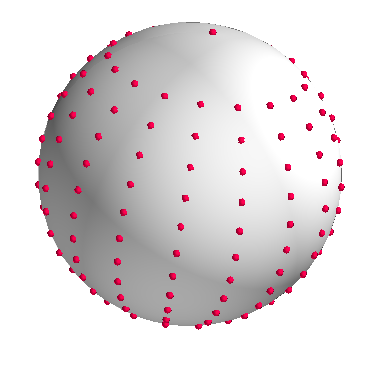
\includegraphics[scale=0.4]{img/gradient_20_9.png}
	\caption{Puntos críticos del gradiente para $n$=20 y $k$=9.}
\end{figure}

\begin{figure}[H]
	\centering
	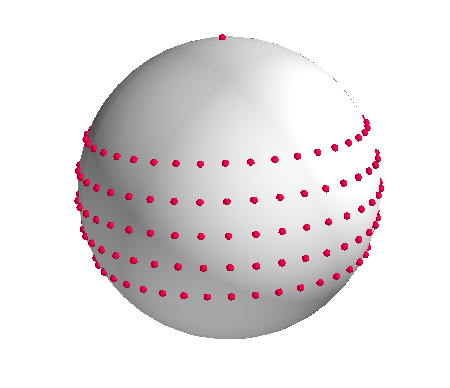
\includegraphics[scale=0.5]{img/gradient_25_5.png}
	\caption{Puntos críticos del gradiente para $n$=25 y $k$=20.}
\end{figure}

\begin{figure}[H]
	\centering
	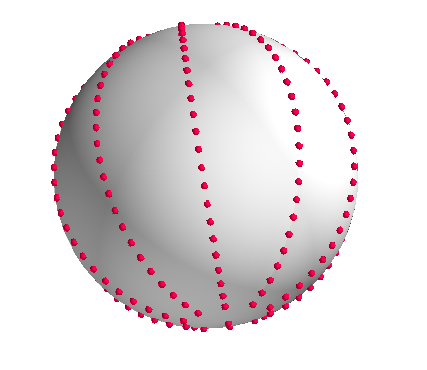
\includegraphics[scale=0.5]{img/gradient_30_5.png}
	\caption{Puntos críticos del gradiente para $n$=30 y $k$=5.}
\end{figure}
 % Calculo del gradiente
\chapter[Integración Numérica]{Integración Numérica}
En este capítulo vamos a obtener una aproximación numérica de la integral $$ I(f) = \int_{\mathds{S}^2} f(\eta) dS^2(\eta). $$. 
\section{Fórmulas de una variable.}
En primer lugar tomaremos la siguientes coordenadas esféricas
$$ \eta \mapsto (\cos\phi \sin\theta, \sin\phi \sin\theta,\cos \theta), \quad 0\le \phi \le 2\pi, 0\le \theta \le \pi$$
 
Ahora, 
$$
I(f) = \int_{0}^{2\pi} \int_{0}^{\pi} f(\cos\phi \sin\theta, \sin\phi \sin\theta,\cos \theta)\sin\theta d\theta d\phi. 
$$

Una vez hemos simplificado la expresión de la integral podemos aplicar métodos de integración numérica de una variable a cada una de las integrales. Comenzaremos integrando respecto a $\phi$.
\medskip
\begin{rem}Regla del trapecio compuesta.
	$$\int_{a}^{b} f(x)dx \approx \frac{b-a}{n}\left[\frac{f(a)+f(b)}{2}+\sum_{k=1}^{n-1}f(a+k\frac{b-a}{n})\right].
	$$
\end{rem}

Como el integrando es periódico en $\pi$ con periodo $2\pi$, usando la regla del trapecio tenemos que

$$
\widetilde{I}(g)\equiv \int_{0}^{2\pi} g(\phi)d\phi \approx \widetilde{I_m}(g) \equiv \frac{2\pi}{m} \sum_{j=1}^{m} g(j\frac{2\pi}{m})
$$

\begin{lem} Para $m\ge 2,k\ge 0$
	
	\begin{gather*}
	\begin{aligned}
	\int_{0}^{2\pi} \cos(k\phi)d\phi &= \left\{\begin{array}{ll} 2\pi, \qquad k=0 
											\\ 0 ,  \qquad\  k>0
		\end{array} 
		\right.
	\\
	\frac{2\pi}{m}\sum_{j=0}^{m-1}\cos(k\frac{2j\pi}{m}) &= \left\{\begin{array}{ll} 2\pi, \qquad k=0,m,2m,... 
	\\ 0 ,  \qquad en\ otro\ caso
	\end{array} 
	\right.
	\\
	\int_{0}^{2\pi} \sen(k\phi)d\phi &=  \frac{2\pi}{m}\sum_{j=1}^{m-1}\sen(k\frac{2j\pi}{m}) =0 
	\end{aligned}
	\end{gather*}
\end{lem}
\begin{proof}
Basta con sustituir las siguientes expresiones en la fórmula del trapecio
\begin{gather*}
\cos(iw) = \frac{e^{iw}+e^{-iw}}{2} \\
\sen(iw) = \frac{e^{iw}-e^{-iw}}{2i}
\end{gather*} 
\end{proof}

Finalmente estudiaremos la convergencia de $\widetilde{I}(g)$ a $I(g)$. Para estudiar la convergencia de funciones periódicas, introduciremos el espacio $H^q(2\pi)$ como aquel de las funciones de cuadrado integrable en $(0,2\pi)$ que verifican que 
$$
||f||_q = \sqrt{|a_0|^2+\sum_{}^{}|k||a_k|^2} < +\infty
$$
siendo $a_k$ los coeficientes de la serie de Fourier.
El espacio $H^q(2\pi)$ es un espacio de Hilbert con el producto escalar 
$$ (f,g)_q = a_0b_0 + \sum_{k=1}^{\infty}|k|^{2q} a_kb_k $$ siendo $a_k,b_k$ los coeficientes de la serie de Fourier para f y g respectivamente. 

\begin{thm}Sean $q > \frac{1}{2}, g\in H^q(2\pi)$, entonces
	$$
	| I(g) - I_m(g) | \le \frac{\sqrt{4\pi\zeta(2q)}}{m^q} ||g||_q, \qquad m\ge 1
	$$  
	siendo $\zeta$ la función zeta de Riemann,
	$$\zeta(s) = \sum_{j=1}^{\infty} \frac{1}{j^s}$$
\end{thm}
%¿demostracion?ref[13,p.316]

Por otro lado, estudiamos el valor de la integral $$\int_{0}^{2\pi} f(\cos\phi \sen\theta,\sen\phi \sin\theta,\cos\theta)\sen\theta d\theta$$. Para ello, hacemos el cambio de variable $z= \cos\theta$, la integral queda:
$$
\int_{-1}^{1} f(\cos\phi\sqrt{1-z^2},\sen \phi\sqrt{1-z^2},z) dz 
$$
\begin{rem}Integración de Gauss-Legendre
	$$
	\int_{-1}^{1}f(x)dx \approx \sum_{i=1}^{n} w_if(x_i)
	$$
\end{rem}
Aplicamos la integración de Gauss-Legendre en $-1<z<1$.
\begin{gather}\label{gaussian_quadrature}
\begin{aligned}
I_n(f) &= h \sum_{j=0}^{2n-1} \sum_{k=1}^{n} w_k f(\cos \phi_j\sqrt{1-z^2}, \sen\phi_j\sqrt{1-z^2},z) \\ &= h \sum_{j=0}^{2n-1} \sum_{k=1}^{n} w_k f(\cos \phi_j\sen\theta_k, \sen\phi_j\sen\theta_k,\cos\theta_k)
\end{aligned}
\end{gather}
siendo ${z_i},{w_i}$ los nodos y los pesos de la fórmula de Gauss-Legendre respectivamente.
\begin{thm}Sea $f$ un polinomio esférico de grado menor o igual a $2n-1$. Entonces $I(f)=I_n(f)$. Además, para $f(x,y,z) = z^{2n}$,$I(f)\neq I_n(f)$
 	
\end{thm}
\begin{proof}
	
	Supongamos $f(x,y,z)= x^ry^sz^t, \quad r+s+t \le 2n-1$. Haciendo el cambio a coordenadas esféricas:
	$$
	I = \int_{\mathds{S}^2} x^ry^sz^t dS^2 = \int_{0}^{2\pi} \int_{0}^{\pi} \cos^r\phi \sen^{r+s+1}\theta \sen^s \phi \cos^t \theta d\phi d\theta
	$$
	Sean 
	\begin{gather*}
	\begin{aligned}
	I &= \int_{\esfera} x^r y^s z^t dU = J^{r,s}K^{r,s,t} \\
	J^{r,s} &= \int_{0}^{2\pi} \cos^r\phi \sen ^s \phi d\phi \\
	K^{r,s,t} &= \int_{0}^{\pi} \sen^{r+s+1} \theta \cos^t \theta d\theta
	\end{aligned}
	\end{gather*}
	Para la correspondiente integral numérica tenemos
	y la correspondiente aproximación numérica
	\begin{gather}
	\begin{aligned}
		I_m &= \sum_{j=1}^{2n} \sum_{k=1}^{n} w_k x_{j,k}^r y_{j,k}^s z_{k}^t = J^{r,s}K^{r,s,t} \\
		J_n^{r,s} &= h \sum_{j=1}^{2n} \cos^r \phi_j \sen^s \phi_j \\
		K_n^{r,s,t} &= \sum_{k=1}^{n} w_k \sen^{r+s+1} \theta_k \cos^t \theta_k
	\end{aligned}
	\end{gather}

	Los valores $\{x_{j,k},y_{j,k},z_k\}$ representan las coordenadas cartesianas de los puntos obtenidos mediante las coordenadas esféricas $\{\phi_j\}$ y $\{\theta_j\}$.
	
	\medskip
	
	Ahora, analizaremos el error, $$ E_n = I-I_n = J^{r,s}K^{r,s,t}- J_n^{r,s}K_n^{r,s,t}$$
	
	Usaremos las siguientes propiedades trigonométicas, suponiendo que $r$ es impar y $s$ es par
	\begin{gather*}
	\begin{aligned}
	\cos^r(\pi+w) &= \cos^r(\pi-w) \\
	\sen^s(\pi+w) &= \sen^s(w) \\
	\sen^s (\frac{\pi}{2}+w) &= \sen^s (\frac{\pi}{2}-w) \\
	\cos^r (\frac{\pi}{2}+w) &= -\cos^r (\frac{\pi}{2}-w)
	\end{aligned}
	\end{gather*}

De estas igualdades se deduce que
\begin{gather*}
\begin{aligned}
J^{r,s} = J_n^{r,s} = 0
\end{aligned}
\end{gather*}
Razonando análogamente se obtiene la misma igualdad cuando $r$ es par y $s$ impar o cuando ambos son impares. En consecuencia $I-I_n = 0$.

\medskip

En \cite[p.170]{libro_esfarm} se demuestra que si  $f(x,y,z) = z^{2n}$ entonces $I(f)\neq I_n(f)$.
\end{proof} 
Finalmente, obtendremos una cota del error. Para ello haremos uso del Teorema 4.5 \cite[p.142]{libro_esfarm} y del corolario del Teorema 4.11 \cite[p.149]{libro_esfarm}.
\medskip

El error minimax de la aproximación de una función $f\in C(\esfera)$ por un polinomio esférico de grado menor o igual a m, se define como 
$$
E_{m,\infty}(f) = \min ||f-p||_{\infty}
$$
Sea $p_m^*$ un polinomio esférico de grado menor o igual a m cuyo error minimax se alcanza. La existencia de $p_m^*$ es consecuencia de los resultados citados anteriormente.
\medskip

De (\ref{gaussian_quadrature}) se deduce que $I(p_{2n-1}^*)=I_n(p_{2n-1}^*)$
Ahora, para $g\in C(\esfera)$
\begin{gather}
|I(g)| \le 4\pi||g||_\infty \\
|I_n(g)|\le 4\pi||g||_\infty
\end{gather}
y
\begin{gather}
I(f) - I_n(f) = I(f-p^*_{2n-1}) - I_n(f-p^*_{2n-1}) \\
|I(f) - I_n(f)| \le | I(f-p^*_{2n-1}) | + |  I_n(f-p^*_{2n-1}) | \le 8\pi||f-p^*_{2n-1}||_\infty
\end{gather}
\section{Métodos de Gauss de Orden Superior.}

En el caso de integración en una variable los métodos gaussianos se basan en pedir que la fórmula sea exacta para polinomios del mayor grado posible. Si tenemos n nodos es posible alcanzar esa exactitud para polinomios de grado $2n-1$. Este enfoque se generaliza para la integración en varias variables. \\
Sea $$
I(f)= \int f(\eta)dS^2(\eta) \approx I_N(f) = \sum_{k=1}^{N} w_kf(\eta_k)$$

Los nodos ${n_k}$, y los pesos ${w_k}$ se eligen de forma que la fórmula sea exacta para los armónicos esféricos de mayor grado posible.

\begin{thm}Sea $\mathcal{G}$ un grupo finito de rotaciones sobre la esfera. Y supongamos que el sistema anterior es invariante para todos los elementos de $\mathcal{G}$, es decir, $I_N(f_\gamma)=I_N(f), \quad \forall \gamma \in \mathcal{G}$. Entonces $$\{\eta_i:i=1,...,N\}=\{\gamma(\eta_i):i=1,...,N\}$$ Además ,para cada nodo $\eta_i$ sea $\mathcal{S}_i=\{\gamma(\eta_i):\gamma \in \mathcal{G}\}$.Entonces los pesos asociados a los nodos son iguales. Es condición necesaria y suficiente que f sea invariante para todo elemento de $\mathcal{G}$ para que  se verifique $I(f)=I_N(f)$. En tal caso, decimos que $I_N(f)$ tiene grado de precisión $d$, siendo $d$ la dimensión de f .

\end{thm}
\begin{proof}
Como la esfera es simétrica por rotaciones se verifica que $$I(f) = \int_{\esfera} f(\eta)dS^2(\eta) = \int_{\esfera} f_\gamma(\eta)dS^2(\eta) = I(f_\gamma)$$.
Sea $f^* = \frac{1}{|\mathcal{G}|} \sum_{\gamma \in |\mathcal{G}| } f\gamma$. $f^*$ es invariante por $\mathcal{G}$ e $I(f) = I(f^*)$. Por hipótesis del teorema, 
$$I(f)-I_N(f) = I(f^*) - I_N(f^*) $$
Por tanto, si queremos que $I(f)=I_N(f)$ para todo polinomio esférico $f$, basta con mostrar que el resultado es cierto para todo polinomio esférico que sea invariante por la acción de  $\mathcal{G}$.
\end{proof}
Razonando análogamente al apartado anterior se prueba que
$$
|I(f)-I_N(d)| \le 8\pi E_d(f)|
$$
y la velocidad con la que $I_N(f)$ converge a $I(f)$ depende de la regularidad de f.
\medskip

Los nodos y los pesos han de ser elegidos de forma que sean invariantes por $\mathcal{G}$. Además, el error $I(f)-I_N(d)$ debe ser 0 para polinomios del mayor grado posible, lo que requiere la resolución de un sistema de ecuaciones no lineal. Estas condiciones hacen que la elección de los nodos y los pesos sea una tarea complicada.
%algo mas?%
%¿meto esto tb?
%\subsection{Eficiencia.}
%\subsection{Método de los centroides}

\section{Integración puntos dispersos}
Supongamos que tenemos N nodos, $P=\{\eta_1,...,\eta_N\}$ y sus valores aproximados $f_i~\approx f(\eta_i)$. Queremos aproximar la integral $I(f) =  \int_{\mathds{S}^2} f(\eta)dS^2(\eta)$.

\medskip
Tomamos $T_N=\{\triangle_1,...,\triangle_{M(N)}\}$ la triangulación de $\mathds{S}^2$, donde los vértices de la triangulación son los nodos.

$$
I(f) = \sum_{k=1}^{M} \int_{\triangle_k} f(n)dS^2(n) \approx  \sum_{k=1}^{M} \frac{1}{3}[f(n_{k,1})+f(n_{k,2})+f(n_{k,3})] area(\triangle_k)
$$
Realizando un análisis del error cometido similar al realizado anteriormente, obtenemos que el método tiene grado de precisión 0 y 
$|I(f)-I_n(f)|\le 4\pi c_f h$ siendo $h=\max$ diam$(\triangle), \quad \triangle\in T_N$
Luego, f es lipschitziana en $\mathds{S}^2$ con constante $ c_f$

Finalmente, se nos plantean dos cuestiones: elegir una triangulación y un conjunto de nodos. Una de las opciones más frecuentes para la primera cuestión es la triangulación de Delaunay. En cuanto al conjunto de nodos, es conocido que se obtienen buenos resultados tomando un conjunto en el que los punto están bien distribuidos.
%meter referencias a otras triangulaciones y otros nodos$

\section{Integración sobre el disco unidad.}
Finalmente, integraremos sobre el disco unidad $\mathds{D}=\{(x,y):x^2+y^2 \le 1\}.$
La semiesfera superior es la imagen de 
$z=\sqrt{1-x^2-y^2} \qquad (x,y)\in \mathds{D}$

\begin{gather*}
\begin{aligned}
&\int_{D}f(x,y,\sqrt{1-x^2-y^2})\sqrt{1+(\frac{\partial z}{\partial x})^2+(\frac{\partial z}{\partial y})^2} dx dy \\ 
&= \int_D f(x,y,\sqrt{1-x^2-y^2})\frac{dx dy}{\sqrt{1-x^2-y^2}}
\end{aligned}
\end{gather*}
	
Por tanto,
\begin{gather*}
\begin{aligned}
&\int_{\mathds{S}^2}f(\eta) dS^2(\eta)  =\\ &\int_D \left[f(x,y,\sqrt{1-x^2-y^2})+f(x,y,-\sqrt{1-x^2-y^2})\right]\frac{dx dy}{\sqrt{1-x^2-y^2}}
\end{aligned}
\end{gather*}  
Es decir, la integración sobre la esfera es equivalente a una integración con pesos sobre el disco unidad.


$$I(f)=\int_{D} f(x,y) dxdy = \int_{0}^{2\pi}\int_{0}^{1} rf(r\cos\theta,r\sen\theta)drd\theta $$
Para integrar sobre $\theta$ usamos la regla del trapecio y para hacerlo respecto de $r$ usamos la integración de Gauss-Legendre al integrando.

$$ I_n(f) = h\sum_{j=0}^{2n}\sum_{j=0}^{n} w_k r_k f(r_k \cos\theta_j,r_k\sen\theta_j)$$
\begin{thm}Sea f(x,y) un polinomio de grado menor o igual a $2n$, entonces $I(f)=I_n(f)$. Además, la fórmula anterior tiene exactitud $2n$. 
\end{thm}
\begin{proof}
	Supongamos $f(x,y)=x^\alpha y^\beta$ con  $\alpha,\beta$ enteros positivos y tales que  $\alpha+\beta \le n$, entonces
	$$
	I(f)=\left(\int_{0}^{2\pi}(\cos\theta)^{\alpha}(\sen\theta)^{\beta}d\theta\right)\left(\int_{0}^{1}r^{\alpha+\beta +1}\right) \equiv J^{\alpha,\beta}K^{ \alpha+\beta+1 }
	$$
	$$
	I_n(f) = \left(h\sum_{j=0}^{2n}(\cos\theta_j)^{\alpha}(\sen\theta_j)^{\beta}\right) \left(\sum_{j=0}^{n}w_kr_k^{\alpha+\beta+1}\right)\equiv J_n^{\alpha,\beta}K_n^{ \alpha+\beta+1 }
	$$
	siendo
	$$
	K^t = \int_{0}^{1 } r^t \qquad K_n^t=\sum_{k=0}^{n} w_k{r_k}^t
	$$
	
	Por otro lado, si $\beta$ es impar las integrales $J^{\alpha,\beta},J_n^{\alpha,\beta}=0$ (visto en la demostración del Teorema 3.5). Si $\beta$ es par podemos transformar el integrando $(\cos \theta)^\alpha(\sen\theta)^\beta$ en un polinomio de potencias de $\cos \theta$ con grado $\alpha+\beta$. Usando el Lema 3.2 se tiene que $J_n^{\alpha,\beta} = J^{\alpha,\beta}, \alpha+\beta\le 2n$. 
	\medskip
	La fórmula de Gauss-Legendre para (n+1) puntos tiene exactitud 2n+1,luego $K_n^{ \alpha+\beta+1 }=K^{ \alpha+\beta+1 }, \quad \alpha+\beta \le 2n$.
	\medskip
	
	Por tanto, hemos probado que $I(f) = I_n(f) \quad \forall \alpha,\beta\ge 0, 0\le\alpha+\beta \le 2n $.
	Para comprobar que $I_n(f)$ tiene exactitud 2n basta considerar la función $f(x,y) = r(r\cos\theta)^{2n+1}$. En este caso, $J^{2n+1,0}=0$ y $J_n^{2n+1,0},K_n^{2n+2}$ no se anulan.
\end{proof} %integracion numerica
\chapter[Kaggle]{Kaggle}
\section{Introducción.}
\subsection{Descripción del problema.}
Los atributos son los siguientes
\begin{itemize}
	\item ip
	\item app
	\item device
	\item so
	\item click\_time
	\item attributed\_time
	\item is\_attributed
\end{itemize}
\subsection{Limitaciones encontradas.}
La principal limitación hardware que he encontrado es el uso de memoria RAM debido al gran tamaño del conjunto de entrenamiento (7.7 GB).
\subsection{Herramientas utilizadas}
Boosting es un enfoque donde el resultado se da usando la media
ponderada de varios árboles y combina las ventajas de cada árbol al darle
a éste un peso en la decisión final. En este enfoque, los árboles tienen
que ir construyéndose de manera lineal para intentar añadir árboles que
mejoren aquello en lo que el resto ha fallado. El objetivo final es eliminar el
sesgo. [9]
Para la competición en particular, se ha usado la librería XGBoost,
que nos permite usar Boosting con árboles de forma paralela, eficiente y
flexible. Este ha sido el algoritmo usado en el resultado final debido a su
capacidad para obtener valores significativamente superiores a Random
Forest, aunque sacrificando velocidad en el entrenamiento.
He usado los siguientes bibliotecas
\begin{itemize}
	\item xgboost
	\item matplotlib
	\item pandas
	\item numpy
\end{itemize}
\section{Objetivos.}
\section{Estudio de los datos.}
Para poder elegir una estrategia para el preprocesamiento es necesario realizar una visualización de los datos. De esta forma, podremos obtener cómo están distribuidos los valores de cada uno de los atributos o si existe alguna relación de correlación entre ellos. Para poder realizar este estudio correctamente separaremos los atributos de tipo fecha en dia,mes y año.
\begin{figure}[H]
	\centering
	\begin{subfigure}{.5\textwidth}
		\centering
		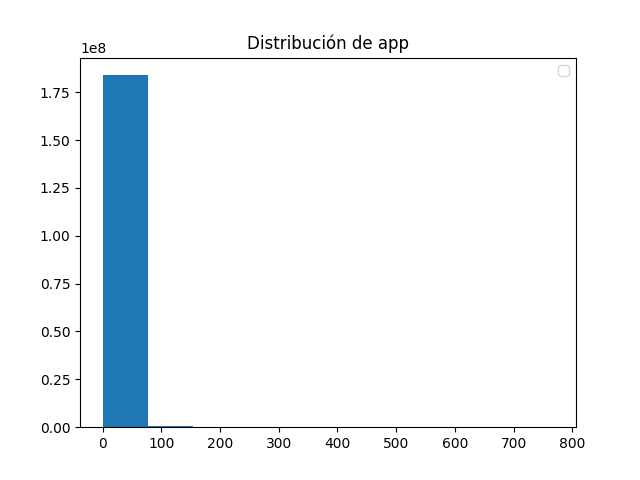
\includegraphics[scale=0.5]{img/app_distribution.png}
		\caption{A subfigure}
		\label{fig:sub1}
	\end{subfigure}%
	\begin{subfigure}{.5\textwidth}
		\centering
		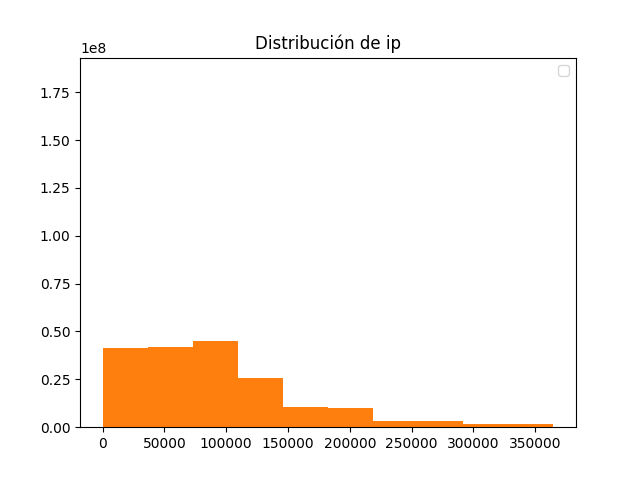
\includegraphics[scale=0.5]{img/ip_distribution.png}
		\caption{A subfigure}
		\label{fig:sub2}
	\end{subfigure}
	\caption{A figure with two subfigures}
	\label{fig:test}
\end{figure}
\begin{figure}[H]
	\centering
	\begin{subfigure}{.5\textwidth}
		\centering
	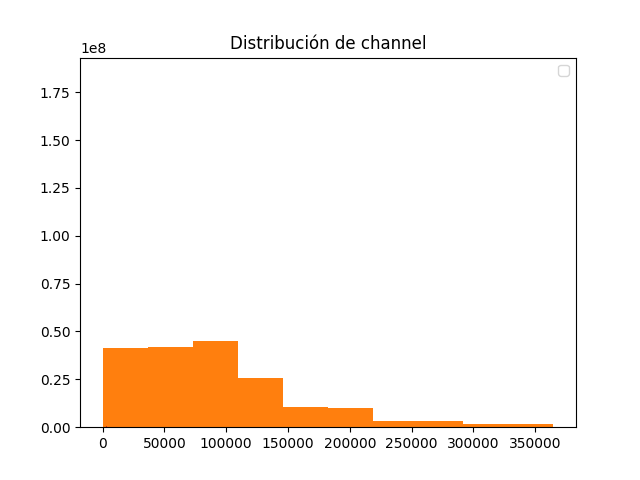
\includegraphics[scale=0.5]{img/channel_distribution.png}
		\caption{A subfigure}
		\label{fig:sub1}
	\end{subfigure}%
	\begin{subfigure}{.5\textwidth}
		\centering
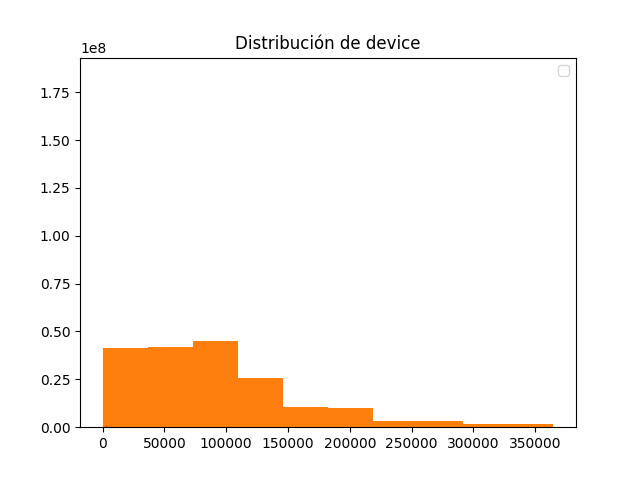
\includegraphics[scale=0.5]{img/device_distribution.png}
		\caption{A subfigure}
		\label{fig:sub2}
	\end{subfigure}
	\caption{A figure with two subfigures}
	\label{fig:test}
\end{figure}

\begin{figure}[H]
	\centering
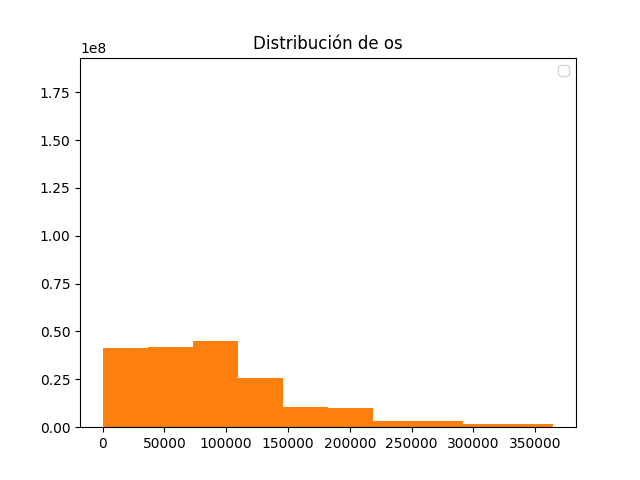
\includegraphics[scale=0.5]{img/os_distribution.png}
\caption{A figure with two subfigures}
\label{fig:test}	
\end{figure}
En las gráficas anteriores podemos observar que las variables app,channel,device,ip y os se d
\medskip
Ahora, estudiaremos la variable click\_time. Al tratarse de una variable que representa una hora y fecha, la dividiremos en día,mes,año y valor timestamp(segundos transcurridos desde una fecha fijada por el sistema operativo).
\begin{figure}[H]
	\centering
	\begin{subfigure}{.5\textwidth}
		\centering
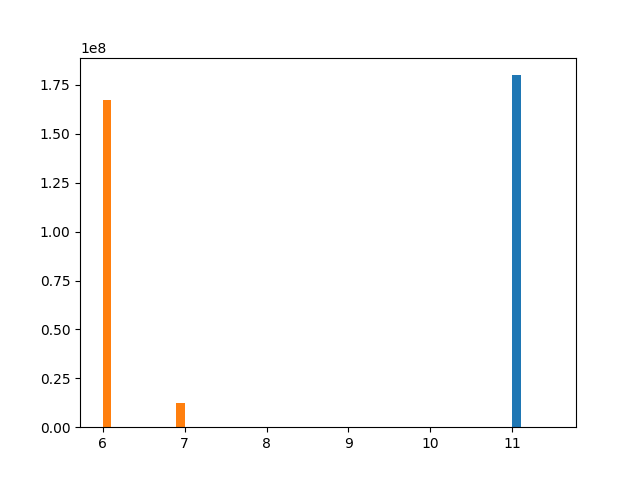
\includegraphics[scale=0.45]{img/click_time_day_distribution.png}
		\caption{A subfigure}
		\label{fig:sub1}
	\end{subfigure}%
	\begin{subfigure}{.5\textwidth}
		\centering
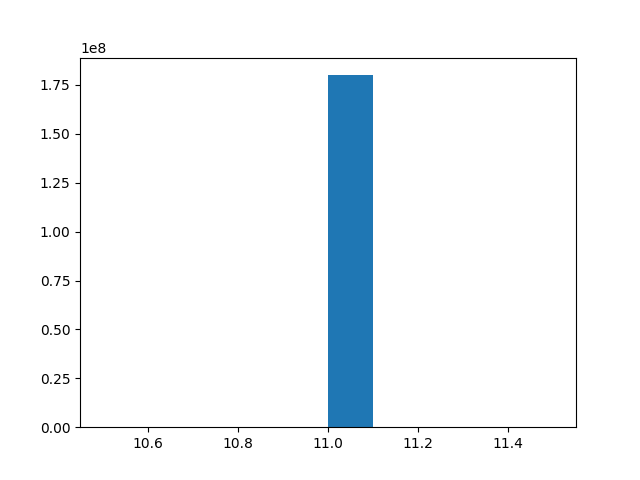
\includegraphics[scale=0.45]{img/click_time_month_distribution.png}
		\caption{A subfigure}
		\label{fig:sub2}
	\end{subfigure}
	\caption{A figure with two subfigures}
	\label{fig:test}
\end{figure}
\begin{figure}[H]
	\centering
	\begin{subfigure}{.5\textwidth}
		\centering
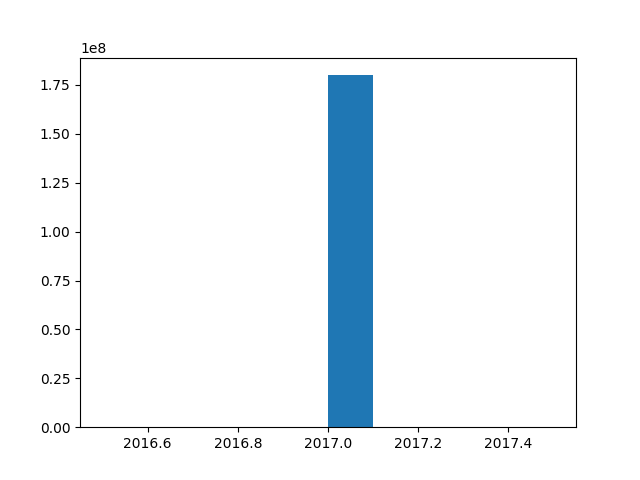
\includegraphics[scale=0.5]{img/click_time_year_distribution.png}
		\caption{A subfigure}
		\label{fig:sub1}
	\end{subfigure}%
	\begin{subfigure}{.5\textwidth}
		\centering
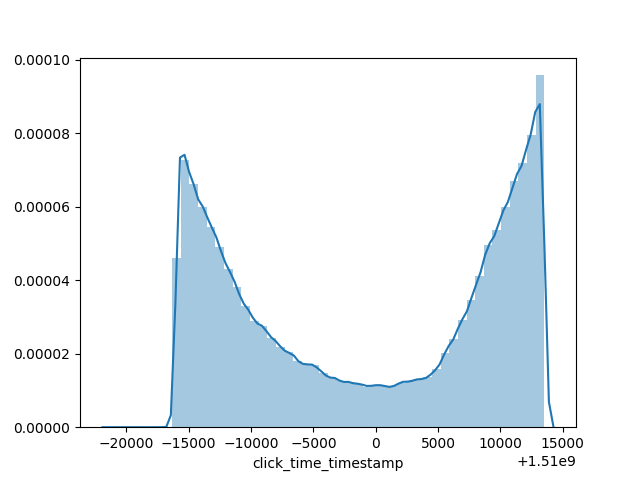
\includegraphics[scale=0.5]{img/normalDistclick_time_timestamp.png}
		\caption{A subfigure}
		\label{fig:sub2}
	\end{subfigure}
	\caption{A figure with two subfigures}
	\label{fig:test}
\end{figure}

En esta ocasión si podemos establecer valores fijos para algunos campos:
\begin{enumerate}
	\item Los días son el 6,7 y 11
	\item Todos los valores corresponden al mes 11.
	\item Todos los registros corresponden al año 2017
\end{enumerate}

Finalmente, estudiaremos el balanceo de clases de la variable a clasificar. Cabe recordar que un desbalanceo de clases provocará que el modelo de aprendizaje que construiremos no clasifica bien para las clases minoritarias.
\begin{figure}[H]
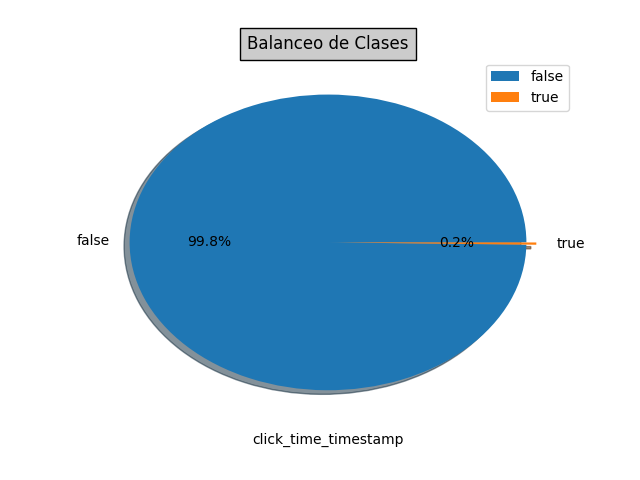
\includegraphics[scale=0.75]{img/imbalacing.png}
\label{}
\caption{Balanceo de clases}
\end{figure}
Por otro lado, estudiaremos el número de valores desconocidos de cada columna ya que un atributo con un gran número de valores desconocidos no nos proporciona información valiosa. Los resultados obtenidos son los siguientes.
\begin{table}[H]
	\centering
	\begin{tabular}{lllll}
	Atributo& Total & \%    \\
	ip	& 0 &0 \\
	app	& 0 & 0   \\
	os	& 0 & 0 \\
	chanel &0 & 0 \\
	device & 0 & 0  \\
	click\_time& 0& 0 \\
	attributed\_time &184447044& 0.997529
	\end{tabular}
	\caption{}
\label{}
\end{table}
\section{Preprocesamiento.}
En este tipo de competiciones la fase de preprocesamiento suele ser la que marca más la diferencia. Esto es debido a que a igualdad de capacidad de procesamiento, se puede obtener la configuración de parámetros óptima para los algoritmos usados, siendo los algoritmos usados similares entre los participantes.
\medskip
Para evaluar la bondad de las decisiones tomadas haremos uso de la clasificación mediante boosting, debido a que nos permite ver la importancia de cada atributo a la hora de construir el modelo de aprendizaje. Esto nos permitirá discriminar que cambios nos proporcionan mejoras.
\medskip
Los resultados obtenidos en la sección anterior nos llevan a tomar las siguientes decisiones:
\begin{itemize}
	\item Eliminar la columna attributed\_time
	\item Eliminar las columnas mes y año provenientes de click\_time
\end{itemize}
A continuación, vamos a  seguir trabajando con la variable click\_time los siguientes cambios a probar son introducir el día de la semana y la hora.
Finalmente, realizaremos algunas agrupaciones añadiendo una columna que contabilize el número de instancias coincidentes:
\begin{itemize}
	\item ip-day-hour
	\item ip-app
	\item ip-app-os	
\end{itemize}
Los resultados obtenidos en las distintas fases de preprocesamiento se muestran en la siguiente tabla.
\begin{table}[]
	\centering
	\caption{My caption}
	\label{my-label}
	\begin{tabular}{lllll}
		Cambio realizado& Resultado & Importancia del cambio introducido &  &  \\
		&  &  &  &  \\
		&  &  &  &  \\
		&  &  &  & 
	\end{tabular}
\end{table}
\section{Soluciones planteadas.}
\subsection{}
Para la búsqueda de los mejores parámetros en cada clasificador, se
aplica el concepto de Grid Search. Esto significa que podemos hacer bucles
para explorar con diferentes valores y combinaciones de parámetros. Si
tenemos suficiente capacidad de procesamiento, es lo ideal a la hora de
optimizar los parámetros, pero, como es de esperar, es una operación muy
pesada.
\subsection{RUSBoosting}
\begin{algorithm}
\end{algorithm}
\subsection{CUSBoosting}
\begin{algorithm}
\end{algorithm}
\subsection{MIX}
\subsection{Resultados obtenidos.}
\section{Conclusiones obtenidas.}
\subsection{Cosas que se quedaron por hacer.}

\appendix

\chapter{La Función Gamma}\label{aped.A}
\begin{defn} Dado $x\in\mathds{(R)^+}$ definimos la función gamma como
	$$
	\Gamma(x) := \int_{0}^{\infty} t^{x-1}e^{-t}dt		
	$$
\end{defn}
\begin{prop}Se verifican las siguientes formulas:
	$$
	\int_{0}^{\infty}  t^{x-1}e^{-at^b}dt = b^{-1}a^{-x/b}\Gamma(x/b)  , x,a,b \in \mathds{R}^+
	$$
	
	$$
	\int_{0}^{1} |ln t|^{x-1}dt = \Gamma(x),   x \in \mathds{R}^+
	$$
	
	$$
	\Gamma(x+1) = x \Gamma(x) ,		x\in \mathds{R}^+
	$$
	
	$$
	\Gamma^{(k)}(x) = \int_{0}^{\infty} (ln t)^k t^{x-1} e^{-t} dt,   k\in\mathds{N}_0,x\in\mathds{R}^+
	$$
\end{prop}
\begin{rem}
	$\Gamma(1)=1$ y de la tercera fórmula se deduce que $\Gamma(n+1)=n!, n\in\mathds{N}_0$. Es decir, la función $\Gamma$ extiende el operador factorial de los números naturales a los reales positivos.
\end{rem}
\begin{lem} 
	$$
	\Gamma(\frac{1}{2}) = 	\sqrt{\pi}
	$$
	$$
	\Gamma(n+\frac{1}{2})=\frac{(2n)!}{2^{2n}n!} \sqrt{\pi}
	$$
\end{lem}
\begin{defn}Sea $x\in\mathds{R}$ y $n\in\mathds{N}$,el símbolo de Pochhammer se define como
	$$
	(x)_0 = 1, (x)_n=x(x+1)(x+2)...(x+n-1)
	$$
\end{defn}
\begin{prop} Sea $x\in\mathds{R}^+$ entonces
	$$
	(x)_n = \frac{\Gamma(x+n)}{\Gamma(x)}
	$$
\end{prop}
\chapter{Resultados básicos de la esfera.}\label{aped.B}
Usaremos $dV^d$ para elemento diferencial de volumen y $dS^{d-1}$ para elemento diferencial de superficie de la esfera.  $\mathds{S^{d-1}}$

\begin{prop}Para $d \ge 3$ y $\xi \in \mathds{S}^{d-1}$,con $\xi_{(d)} = te_d+\sqrt{1-t^2}\xi_{(d-1)},  t\in[-1,1]$ , se tiene que
	$$
	dS^{d-1}(te_d+\sqrt{1-t^2}\xi_{(d-1)}) = (1-t^2)^{\frac{d-3}{2}}dt  dS^{d-2}(\xi_{(d-1)})
	$$
	Equivalentemente,
	$$
	dS^{d-1} = (1-t^2)^{\frac{d-3}{2}}dt dS^{d-2}
	$$
\end{prop}
\begin{example}Sea d=3 y $\xi$ un punto genérico de la esfera. Usando coordenadas esféricas $$
	\xi_{(3)}=\begin{pmatrix}
	cos\phi sen\theta\\
	sen\phi sen\theta\\
	cos\theta\\
	\end{pmatrix}
	0 \le \phi \le 2\pi , 0 \le \theta \le \pi
	$$
	Sea $t=cos\theta$ entonces
	$$
	\xi_{(2)} = \begin{pmatrix}
	cos\phi\\
	sen\phi\\
	0\\
	\end{pmatrix}
	$$
	Por tanto,$ \xi_{(3)} = te_3 + \sqrt{1-t^2} \xi_{(2)}$ y $dS^1 = d\phi , dS^2 = dtd\phi$
	
\end{example}
Podemos usar la anterior proposición para el cálculo del área de la superficie de la esfera.
\begin{prop}Se verifica que
	$$
	|\mathds{S}^{d-1}| = \int_{\mathds{S}^{d-1}} dS^{d-1} = \frac{2\pi^\frac{d}{2}}{\Gamma(\frac{d}{2})}
	$$
\end{prop} 

\begin{prop}
	Sea $A\in\mathds{R}^{dxd}$ ortogonal entonces
	$$ dS^{d-1}(A\xi) =  dS^{d-1}(\xi)$$
	$$ dV^{d}(A\xi) =  dV^{d}(\xi)$$
\end{prop}

Llamamos $C(S^{d-1})$ al espacio de funciones continuas sobre  $S^{d-1}$. Este espacio es un espacio de Banach con la norma $ ||f||_\infty = sup \{ |f(\xi) : \xi\in \mathds{S}^{d-1}\}$. Llamaremos $L^2(S^{d-1})$ al espacio de funciones con cuadrado integrable en $S^{d-1}$. Dicho espacio es un Hilbert con el producto escalar$$ (f,g) = \int_{S^{d-1}} f\overline{g} dS^{d-1}
$$
Consideramos el espacio $C(S^{d-1})$ con la norma inducida por el producto escalar de $L^2(S^{d-1})$. Este espacio no es completo. Además, el cierre de $C(S^{d-1})$ respecto a dicha norma es $L^2(S^{d-1})$. Es decir, dado una función $f\in L^2(S^{d-1})$ existe una sucesión $\{f_n\} \subset C(S^{d-1})$ tal que ${f_n}\to f$

\begin{prop}Sean $\Omega_\delta = \{x\in\mathds{R}^d : |x|\in[1-\delta,1+\delta]\}$ y $f^*(x)= f(\frac{x}{|x|}),x\in\Omega_\delta$ y $k\in\mathds{N}$.Entonces $f$ es k veces diferenciable en $S^{d-1}$ cuando $f^*$ lo es.  
\end{prop}
\begin{defn}Definimos $C^k(S^{d-1}), k\in\mathds{N}\cup0$ como el espacio de funciones k veces diferenciables en $S^{d-1}$
\end{defn}
\begin{prop}$C^k(S^{d-1})$ es un espacio de Banach con la norma 
	$$
	||f||_{C^k(S^{d-1})} = ||f^*||_{C^k(\Sigma_\delta)}
	$$
\end{prop}
\begin{rem}Usaremos $||f||_\infty = ||f||_{C(S^{d-1})}$
	
\end{rem}
\chapter{Polinomios de Legendre}\label{aped.C}
\section{Fórmulas de Representación}
\subsection{Fórmula de Rodrigues}
\begin{thm}
	$$P_{n,d}(t) = (-1)^n \frac{\Gamma(\frac{d-1}{2}) }{2^n\Gamma(n+\frac{d-1}{2})}(1-t^2)^{\frac{3-d}{2}}(\frac{d}{dt})^n (1-t^2)^{n+\frac{d-3}{2}}, \quad d\ge2
	$$
\end{thm}
\begin{rem}\label{cte_Rod}
	A la constante $R_{n,d} = \frac{\Gamma(\frac{d-1}{2})}{2^n\Gamma(n+\frac{d-1}{2})}$ se le llama constante de Rodrigues
\end{rem}
\begin{example}
	\begin{itemize}
		\item Si d = 2, $$P_{n,2}(t) = (-1)^n \frac{2^n n!} {(2n)!}(1-t^2)^{\frac{1}{2}}(\frac{d}{dt})^n (1-t^2)^{n-\frac{1}{2}}, \quad n\in \mathds{N}_0$$ Una forma reducida se obtiene usando el polinomio de Chebyshev obteniendo que $P_{n,2}(t) = cos(n \quad arccos t), t\in[-1,1]$
		\item Si d=3, $$P_{n,3}(t) = \frac{1} {2^n n!}(\frac{d}{dt})^n (t^2-1)^{n}, \quad n\in \mathds{N}_0$$
	\end{itemize}
\end{example}
\subsection{Fórmulas de Representación Integral.}
\begin{thm}Sea $n\in\mathds{N}_0$ y $d\ge3$, $$ 
	P_{n,d}(t) = \frac{|\mathds{S}^{d-3}|}{|\mathds{S}^{d-2}|}\int_{-1}^{1}[t+i(1-t^2)^{\frac{1}{2}}s]^n(1-s^2)^{\frac{d-4}{2}} ds, \quad t\in[-1,1]
	$$
\end{thm}
\begin{rem}Como consecuencia de la fórmula anterior se tiene que $P_{n,d}(-t) = (-1)^n P_{n,d}(t), t\in[-1,1]$, es decir $P_{n,d}(t)$ tiene la misma paridad que $n$.
\end{rem}
Podemos obtener otra fórmula de representación integral, usando funciones trigonométricas mediante el cambio de variable $s = tanh(u), u\in\mathds{R}$
\begin{thm}Sea $n\in\mathds{N}_0$ y $d\ge3$, $$
		P_{n,d}(t) = \frac{|\mathds{S}^{d-3}|}{|\mathds{S}^{d-2}|}\int_{-1}^{1}\frac{(1-s^2)^{\frac{d-4}{2}}}{[t\pm i(1-t^2)^{\frac{1}{2}}s]^{n+d-2}} ds, \quad t\in(0,1]
	$$
\end{thm}
\section{Propiedades}
\begin{prop}
Si $f\in C^n([-1,1])$ entonces 
$$
\int_{-1}^{1} f(t)P_{n,d}(t)(1-t^2)^{\frac{d-3}{2}} dt = R_{n,d}\int_{-1}^{1} f^{(n)}(t)(1-t^2)^{n+\frac{d-3}{2}} dt
$$
siendo $R_{n,d}$ la constante de Rodrigues \hyperref[]{(Nota \ref{cte_Rod})}
\end{prop}
\begin{prop}$P_{n,d}(t)$ tiene n raíces distintas en (-1,1)
\end{prop}
\begin{prop}Los polinomios de Legendre satisfacen la siguiente relación de recurrencia
	\begin{gather*}
		P_{n,d}(t) = \frac{2n+d-4}{n+d-3}t	P_{n-1,d}(t) - \frac{n-1}{n+d-3}P_{n-2,d}(t), \qquad n\ge 2, d\ge2 \\
		P_{0,d}(t) = 1 , 	P_{1,d}(t) = t 
	\end{gather*}
\end{prop}
\begin{prop}
	\begin{gather*}
	(1-t^2)P'_{n,d}(t) = n[P_{n-1,d}(t)-tP_{n,d}(t)], \quad n \ge 1,d \ge 2, t \in [-1,1]
	\end{gather*}
\end{prop}
\begin{prop}Para $d\ge 2$
$$\sum_{n=0}^{\infty} N_{n,d}r^nP_{n,d}(t) = \frac{1-r^2}{(1+r^2-2rt)^\frac{d}{2}},\quad |r| < 1, t\in[-1,1] 
$$
\end{prop}
\begin{prop}
	\begin{gather*}
	P_{n,d}(0) = \frac{|\mathds{S}^{d-3}|}{|\mathds{S}^{d-2}|}\int_{-1}^{1} i^n s^n(1-s^2)^{\frac{d-4}{2}}ds \\
	P_{n,d}(-1) = (-1)^n
	\end{gather*}
\end{prop}
\begin{prop}
	$$
	|P_{n,d}(t)| < \frac{\Gamma(\frac{d-1}{2})}{\sqrt{\pi}}\left[\frac{4}{n(1-t^2)}\right]^{\frac{d-2}{2}},\quad n\in\mathds{N}_0,d\ge2,t\in(-1,1)$$
\end{prop}

\chapter{Polinomios de Gegenbauer}\label{aped.D}

\begin{defn}Sean $v\ge 0,n\in\mathds{N}_0$ se define el polinomio de Gegenbauer de grado n e índice v, como:
	$$C_{n,v}(t) = \binom{n+2v-1}{n}\frac{\Gamma(v+\frac{1}{2})}{\sqrt{\pi}\Gamma(v)}\int_{-1}^{1}\left[t+i(1-t^2)^{1/2}s\right]^n (1-s^2)^{v-1} ds$$ 
\end{defn}

\begin{prop}\label{geb_rel}Se verifica la siguiente relación
	$$C_{n,\frac{d-2}{2}}(t) = \begin{pmatrix}
	n+d-3 \\
	b
	\end{pmatrix} P_{n,d}(t)
	$$
\end{prop}
\begin{prop}(Identidad de Gegenbauer.)$$
	\sum_{n=0}^{\infty} C_{n,v}(t) = \frac{1}{(1+r^2-2rt)^v}, \qquad |r|<1, t\in[-1,1]$$
\end{prop}
\begin{prop}\label{propGg} Se verifican las siguientes igualdades:
	\begin{enumerate}[(i)]
	\item $(1-x^2) \frac{d}{dx} C_{n,v}(x) = 2\lambda C_{n,\lambda+1}(x)$
	\item $nC_{n,\lambda}(x) = x\frac{d}{dx} C_{n,\lambda}(x) - \frac{d}{dx} C_{n-1,\lambda}(x)$
	\item $(n+2\lambda) C_{n,\lambda}(x)  = \frac{d}{dx}C_{n,\lambda+1}(x)-x \frac{x}{dx}C_{n,\lambda}(x) \quad n\ge 0$
	\item $\begin{aligned}
		\frac{d}{dx} C_{n+1,\lambda}(x) - C_{n-1,\lambda}(x)  &= 2(n+\lambda)C_{n,\lambda}(x)\\ &= 2\lambda C_{n,\lambda+1}(x) - C_{n-2,\lambda+1}(x) \quad n\ge 1
	\end{aligned}$        	
\end{enumerate}
\end{prop}
\chapter{Funciones de Legendre Asociadas}\label{aped.E}

Las funciones asociadas de Legendre nos permiten construir esféricos armónicos a partir de otros de menor dimensión.
\begin{defn}Sea $d\ge3$ y $n,j \in \mathds{N}_0$ se define la función asociada de Legendre de grado n y orden j en dimensión d, como
	$$
	P_{n,d,j}(t) = \frac{|\mathds{S}^{d-3}|}{|\mathds{S}^{d-2}|}i^{-j} \int_{-1}^{1}\left[t+i(1-t^2)^{1/2}s\right]^n P_{j,d-1}(s)(1-s^2)^{\frac{d-4}{2}}, \quad t\in[-1,1]
	$$
\end{defn}
\begin{rem}Si $j=0, P_{n,d,0}(t)=P_{n,d}(t)$
\end{rem}
%Las funciones asociadas de Legendre nos permiten generar "sistemas" de esféricos armónicos en la esfera.
\begin{prop}Sea $d\le3$ y $0\le j \le n$ 
	$$	P_{n,d,j}(t) = \frac{n!\Gamma(\frac{d-1}{2})}{2^j(n-j)!\Gamma(j+\frac{d-1}{2})}(1-t^2)^{1/2} P_{n-j,d+2j}(t), t\in[-1,1]$$
\end{prop}
El siguiente resultado nos proporciona una relación entre las funciones asociadas de Legendre y las derivadas de los polinomios de Legendre.
\begin{prop}Sea $d\le3$ y $0\le j \le n$ 
	$$	P_{n,d,j}(t) = \frac{(n+d-3)!}{(n+j+d-3)!}(1-t^2)^{1/2} P^{(j)}_{n,d}(t), t\in[-1,1]$$
\end{prop}
\begin{prop}
	\begin{gather*}
	\int_{-1}^{1} P_{m,d,j}(t)P_{n,d,j}(t)(1-t^2)^{\frac{d-3}{2}} dt = 0, \qquad m \neq n
	\end{gather*}
\end{prop}
\begin{prop} Las funciones $\tilde{P}_{n,d,j}$ definidas como
	\begin{gather*}
	\tilde{P}_{n,d,j}(t) = \frac{[(2n+d-2)(n-j)!(n+d+j-3)!]^{1/2}}{2^{\frac{d-2}{2}n!\Gamma(\frac{d-1}{2})}}P_{n,d,j}(t), \quad t\in[-1,1]
	\end{gather*}
	están normalizadas, es decir $\int_{-1}^{1} [	\tilde{P}_{n,d,j}]^2(1-t^2)^\frac{d-3}{2} dt = 1$
\end{prop}
\begin{rem}\label{note:fun_leg}Las funciones $	\tilde{P}_{n,d,j}$ pueden ser escritas en función de las derivadas de los polinomios de Legendre 
	\begin{gather*}
	\tilde{P}_{n,d,j}(t) =\frac{(n+d-3)!}{n!\Gamma(\frac{d-1}{2})} \frac{[(2n+d-2)(n-j)!]^{1/2}}{2^{d-2}(n+d+j-3)!}(1-t^2)^{j/2}P^{(j)}_{n,d}(t), \quad t\in[-1,1]
	\end{gather*}
\end{rem}
\chapter{El problema de clasificación}\label{aped.F}
El problema de clasificación consiste en predecir la clase a la que pertenece una instancia basándonos en una serie de características disponibles. Es un tipo de aprendizaje supervisado, es decir, se conoce de antemano la clases a las que pertenecen los ejemplos usados para construir el clasificador.
%meter grafikito%
El proceso de clasificación consta de las siguientes etapas:

\begin{enumerate}
	\item \textbf{Construir el clasificador}. A partir de un conjunto de ejemplos ya clasificados. El modelo resultante establece 
	\item \textbf{Validación}. Se usa un conjunto distinto al de entrenamiento ya clasificado. Para cada instancia de este conjunto se compara el valor devuelto con el valor real.
\end{enumerate}

Una de las técnicas para realizar la evaluación del modelo es la conocida como validación cruzada. Esta técnica consiste en dividir el conjunto de entrenamiento en k partes, usando k-1 partes para construir el clasificador y usar la restante para validar. Este proceso se repite durante k iteraciones de forma que cada parte es usada como conjunto de prueba. Finalmente, se ponderan los resultados de cada iteración para obtener el resultado final.
\begin{figure}
	\centering
	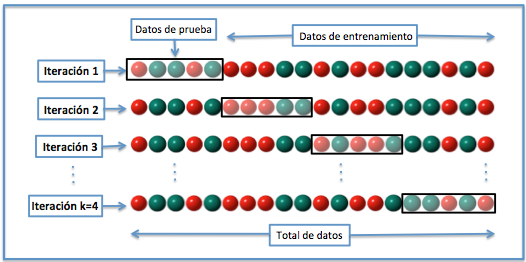
\includegraphics[scale=0.45]{img/K-fold_cross_validation.jpg}
	\caption{Ejemplo validación cruzada.}
\end{figure}
%referencia https://es.wikipedia.org/wiki/Validaci%C3%B3n_cruzada#/media/File:K-fold_cross_validation.jpg

%\begin{thebibliography}{100}
\addcontentsline{toc}{chapter}{Bibliograf\'{\i}a}


\bibitem{At3} 
K.~E. Atkinson,
\newblock {\it An introduction to Numerical Analysis}, 2nd ed.,
\newblock Wiley, New York, 1989.

\bibitem{BF} 
L.~R. Burden, D.~J. Faires,
\newblock {\it An\'alisis Num\'erico}, S\'eptima Edici\'on,
\newblock Thomson Learning, M\'exico, 2003.


\bibitem{Ga13} 
W. Gautschi,
\newblock{\it Numerical analysis}, 2nd ed.,
\newblock Birkh\"auser--Science Springer, New York Dordrecht Heidelberg London 2012.

\bibitem{KCh}
D. Kincaid, W. Cheney,
\newblock {\it  An\'alisis Num\'erico. Las matem\'aticas del c\'alculo
cient\'{\i}fico},
\newblock Addison--Wesley Iberoamericana, Wilmington, 1994.

\bibitem{Ra} 
A. Ralston,
\newblock {\it Introducci\'on al An\'alisis Num\'erico},
\newblock Limusa--Wiley, M\'exico, 1970.

\bibitem{stewart} 
G. W. Stewart,
\newblock {\it Afternotes on Numerical Analysis},
\newblock SIAM, Philadelphia, 1996.

\bibitem{SB} 
J. Stoer, R. Burlirsch,
\newblock {\it Introduction to numerical analysis}, 3rd. ed.,
\newblock Springer, New York, 2002.

\end{thebibliography}




\end{document}

